\chapterimage{chapter_head_2.pdf} % Chapter heading image



\chapter{Percepção musical}
\label{cap:percepcaomusical}

\begin{definition}[Percepção musical:] 
\index{Musicalidade!Percepção musical}
\label{def:PercepcaoMusical}
Esta acontece, quando o dançarino tem um estado de ``sensibilidade'' ou ``conhecimento'' para contemplar ou entender a música,
e assim quando este dança, ``demostrar'' uma coerência entre a música e o que está dançando.
\end{definition}


\newpage

\section{Texturas na música}
\index{Música!Texturas}
\label{sec:texturasmusica}
\begin{wrapfigure}{r}{0.33\textwidth}
    \centering 
    \vspace{-10pt}
    \includegraphics[width=0.30\textwidth]{chapters/cap-musicalidade-percepcion/textura.jpg}
  \caption{Texturas.}
    \vspace{-10pt}
\end{wrapfigure}
De forma similar a como descrevemos a textura numa superfície,
podemos explicar a textura na música.
A textura musical é um termo usado para indicar o modo em que interagem e 
se misturam várias linhas melódicas \cite[pp. 29]{kerman2015listen}.


O termo textura usado na música, 
implica que esta é composta por instrumentos com a capacidade de gerar tons,
e consequentemente melodias;
dado que a percussão não é geralmente considerada como melódica, 
esta não é tomada em conta quando usamos o termo textura \cite[pp. 59]{holland2013music}.

Na música atual existem  vários tipos de texturas, 
porém 3 destes tipos  são os mais comuns 
\cite[pp. 77]{copland1974ouvir} \cite[pp. 29]{kerman2015listen} \cite[pp. 322]{harnum2009basic}:
\begin{inparaitem}
\item textura monofônica, 
\item textura homofônica e
\item textura polifônica.
\end{inparaitem}

 
%%%%%%%%%%%%%%%%%%%%%%%%%%%%%%%%%%%%%%%%%%%%%%%%%%%%%%%%%%%%%%%%%%%%%%%%%%%%%%%%
\subsection{A textura monofônica}
\label{subsec:monofonica}
\index{Música!Monofônica}
\begin{wrapfigure}{r}{0.33\textwidth}
\centering
    \vspace{-10pt}
    \includegraphics[width=0.31\textwidth]{chapters/cap-musicalidade-percepcion/monofonica1.eps}
  \caption{Textura monofônica.}
\end{wrapfigure}
Este tipo de música tem uma única linha melódica sem acompanhamento.
Consequentemente este tipo de música é a mais simples de ouvir, 
pois nossa atenção cai sobre uma única camada na música \cite[pp. 77]{copland1974ouvir} \cite[pp. 29]{kerman2015listen}.
A música monofônica corresponde ao tipo mais antigo de música \cite[pp. 539]{apel1969harvard}.
Se considera que é uma textura monofônica, mesmo que sejam muitas vozes as que executem uma mesma melodia, 
ou que estas executem a mesma melodia em oitavas diferentes \cite[pp. 42]{bennett1993elementos} \cite[pp. 58]{holland2013music}.

A qualificação de textura  monofônica não é afetada pelo uso de instrumentos de percussão tocando junto com a melodia;
a textura monofônica refere-se à parte tonal da música, é dizer à melodia, 
não à textura rítmica da música \cite[pp. 58]{holland2013music}.

\begin{example}
A Figura \ref{fig:ex:monofonica} mostra um exemplo de uma seção de música com textura monofônica.
\end{example}

\begin{figure}[!h]
\centering
    \href{https://drive.google.com/file/d/1o2xCKp2U40Yl28d-GyAbq_llg13Uv5sz/view?usp=sharing}{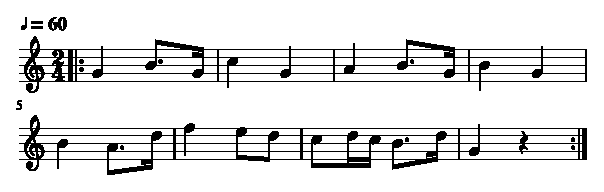
\includegraphics[width=0.99\textwidth]{chapters/cap-musicalidade-percepcion/textura-monofonica-1.eps}}
  \caption{Textura monofônica.}
\label{fig:ex:monofonica}
\end{figure}
 
\begin{example}
Um exemplo, no ocidente,  muito depurado de música monofônica é o canto gregoriano
\cite[pp. 77]{copland1974ouvir} \cite[pp. 29]{kerman2015listen} \cite[pp. 58]{holland2013music}. 
Aqui, não importa o número de vozes usadas na interpretação,
pois todas seguem a mesma linha melódica, pelo que é considerada uma textura monofônica.
\end{example}

%monodia \cite[pp. 38]{schurmann1989m} 

%%%%%%%%%%%%%%%%%%%%%%%%%%%%%%%%%%%%%%%%%%%%%%%%%%%%%%%%%%%%%%%%%%%%%%%%%%%%%%%%
\subsection{A textura homofônica}
\label{subsec:homofonica}
\index{Música!Honofônica}
\begin{wrapfigure}{r}{0.33\textwidth}
  \centering
    \includegraphics[width=0.31\textwidth]{chapters/cap-musicalidade-percepcion/honofonica1.eps}
  \caption{Textura homofônica.}
\end{wrapfigure}
O termo ``homofônico'' ou ``homofonia'' significa literalmente ``vozes semelhantes''.%% Falta referença
A textura homofônica consiste de uma linha melódica principal e um acompanhamento por acordes,
de modo que existe uma distinção clara entre a melodia e a harmonia de acompanhamento;
esta textura é o tipo  mais usado na música atual,
e só é ligeiramente mais complexa que a textura monofônica 
\cite[pp. 78]{copland1974ouvir} \cite[pp. 29]{kerman2015listen} 
\cite[pp. 43]{bennett1993elementos} \cite[pp. 58]{holland2013music}.


A homofonia é o oposto da polifonia, 
pois na textura homofônica só uma linha melódica é importante,
enquanto que na textura polifônica todas as partes contribuem equitativamente para gerar o tecido musical
\cite[pp. 687]{apel1969harvard}.

\begin{example}
A Figura \ref{fig:ex:homofonica} mostra um exemplo de uma seção de música com textura homofônica.
\end{example}

\begin{figure}[!h]
\centering
    \href{https://drive.google.com/file/d/11VBw8pTGFqF-PBofFWZvbqwkfXB56Bfy/view?usp=sharing}{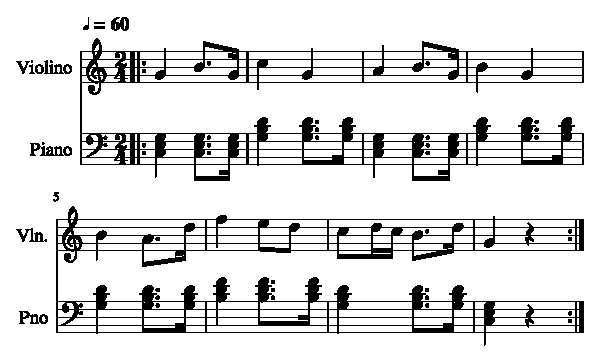
\includegraphics[width=0.99\textwidth]{chapters/cap-musicalidade-percepcion/textura-homofonica-1.eps}}
  \caption{Textura homofônica.}
\label{fig:ex:homofonica}
\end{figure}

\begin{example}
Um exemplo de textura homofônica pode ser visto no choro ``Deixe o breque pra mim'',
de Altamiro Carrilho, 
onde a melodia principal é feita por um único instrumento (flauta), 
com uma base harmônica e percussiva, de acompanhamento.
\end{example}

%\cite[pp. 121]{schurmann1989m} 


%%%%%%%%%%%%%%%%%%%%%%%%%%%%%%%%%%%%%%%%%%%%%%%%%%%%%%%%%%%%%%%%%%%%%%%%%%%%%%%%
\subsection{A textura polifônica}
\index{Música!Polifônica}
\label{subsec:polifonica}
\begin{wrapfigure}{r}{0.33\textwidth}
\centering
    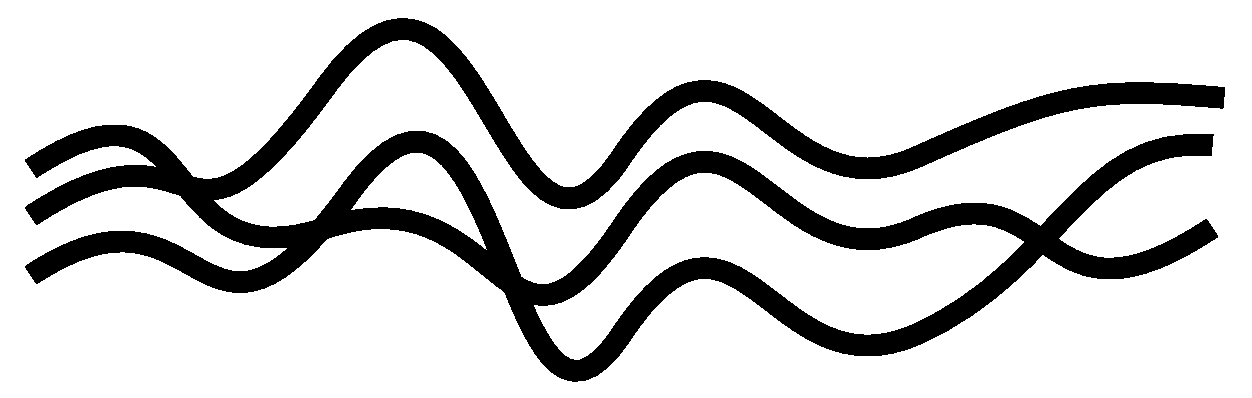
\includegraphics[width=0.31\textwidth]{chapters/cap-musicalidade-percepcion/polifonica1.eps}
  \caption{Textura polifônica.}
\end{wrapfigure}
Termo proveniente do grego, que significa ``vozes múltiplas''.%% Falta referença
A música com textura polifônica se carateriza por ter duas ou mais linhas melódicas  
que se entrelaçam continuamente;
as melodias são consideradas independentes e de interesse aproximadamente igual.
A percepção da música polifônica precisa de um maior nível de atenção 
em comparação das texturas monofônica e homofônica,
pois exige ao ouvinte a capacidade de separar mentalmente cada linha melódica  
\cite[pp. 79-80]{copland1974ouvir} \cite[pp. 29]{kerman2015listen} 
\cite[pp. 42]{bennett1993elementos} \cite[pp. 59]{holland2013music}
\cite[pp. 687]{apel1969harvard}.

Uma termo frequentemente usado na música polifônica é o contraponto;
que é a técnica de escrever duas ou mais melodias que se encaixam 
\cite[pp. 29]{kerman2015listen} \cite[pp. 42]{bennett1993elementos}.

\begin{tcbinformation}{Quantas vozes independentes pode captar simultaneamente um ser humano?}
\label{ref:quantasvozes}
Não existe um senso comum, porém pode-se afirmar que treinando um pouco,
é possível perceber independentemente 2 ou 3 vozes sendo executadas em simultâneo \cite[pp. 81]{copland1974ouvir}. 
\end{tcbinformation} 

\begin{example}
Um exemplo de textura homofônica pode ser visto na música ``Canto e Contraponto'',
de Toquinho e Vinícius, 
onde temos uma melodia executada pela voz, e outra melodia executada por um instrumento fazendo o contraponto, 
com uma base harmônica de acompanhamento.
\end{example}

\begin{example}
A Figura \ref{fig:ex:polifonica} mostra um exemplo de uma seção de música com textura polifônica.
\end{example}

\begin{figure}[!h]
\centering
    \href{https://drive.google.com/file/d/1l-wd3TieQuacMAtdsNI6Z02YubePIGEV/view?usp=sharing}{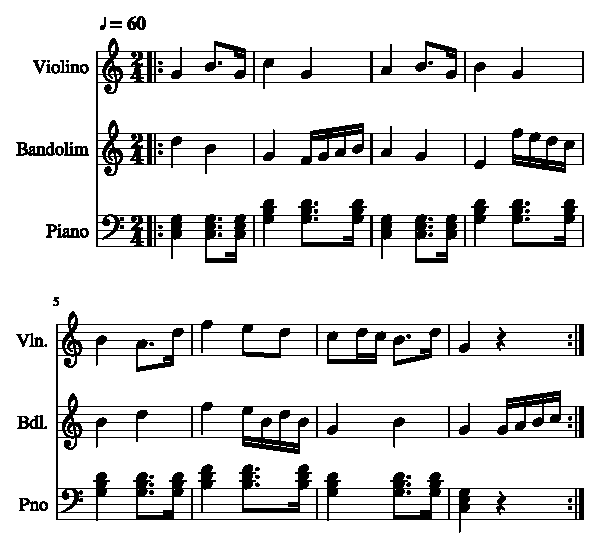
\includegraphics[width=0.99\textwidth]{chapters/cap-musicalidade-percepcion/textura-polifonica-1.eps}}
  \caption{Textura polifônica.}
\label{fig:ex:polifonica}
\end{figure}



%\cite[pp. 64]{schurmann1989m} 

%%%%%%%%%%%%%%%%%%%%%%%%%%%%%%%%%%%%%%%%%%%%%%%%%%%%%%%%%%%%%%%%%%%%%%%%%%%%%%%%
\subsubsection{Polirritmia}
\index{Música!Polirritmia}
\label{subsec:polirritmia}
A polirritmia é a superposição de dois ou mais ritmos.
A polirritmia acontece quando se executam musicas com texturas polifônicas ou homofônicas
\cite[pp. 93]{alves2004teoria};
ou quando vários instrumentos de percussão tocam ritmos diferentes simultaneamente \cite[pp. 35]{holland2013music}.
Assim, a textura dos ritmos simultâneos é chamada polirritmia \cite[pp. 35]{holland2013music}.

Cada instrumento de percussão ``fala'' um ritmo único que geralmente guia os passos e movimentos dos dançarinos;
por exemplo, a música africana é conhecida por ter múltiplas camadas de ritmo e sincopas,
 que são usadas continuamente pelos dançarinos \cite[pp. 35]{holland2013music}.


É possível distinguir dois tipos de polirritmia \cite[pp. 687]{apel1969harvard}:
\begin{itemize}
\item Ritmos contrastantes dentro da mesma \hyperref[def:Metrica]{\textbf{métrica}};
por exemplo, os ritmos mostrados na Figura \ref{fig:polirritmia1-1}.
\begin{figure}[!h]
\centering
    \href{https://drive.google.com/file/d/1uBNMYazV83ynLyp1s6EtsPLb57Xpi9o6/view?usp=sharing}{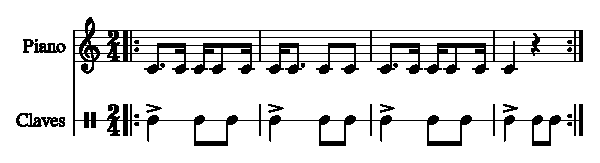
\includegraphics[width=\textwidth]{chapters/cap-musicalidade-percepcion/polirritmia1-1.eps}}
  \caption{Textura polirrítmica com a mesma métrica.}
\label{fig:polirritmia1-1}
\end{figure}
\item Ritmos contrastantes com diferente \hyperref[def:Metrica]{\textbf{métrica}} ou acentuações, 
às vezes é denominado ``polimétrico'';
por exemplo, os ritmos mostrados na Figura \ref{fig:polirritmia2-1}.
\begin{figure}[!h]
\centering
    \href{https://drive.google.com/file/d/1C5Gq4U6rIs7Re2NcdUmVxdHt6qy0CCeX/view?usp=sharing}{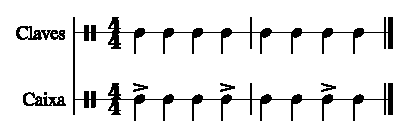
\includegraphics[width=0.7\textwidth]{chapters/cap-musicalidade-percepcion/polirritmia2-1.eps}}
  \caption{Textura polirrítmica com diferente métrica.}
\label{fig:polirritmia2-1}
\end{figure}
\end{itemize}




%%%%%%%%%%%%%%%%%%%%%%%%%%%%%%%%%%%%%%%%%%%%%%%%%%%%%%%%%%%%%%%%%%%%%%%%%%%%%%%%
\section{Percepção da métrica na música}
\label{sec:percepcionmetrica}
Como foi explicado na Pag. \pageref{def:Metrica}, 
a \hyperref[def:Metrica]{\textbf{métrica}} é um padrão ordenado de \hyperref[sec:Tempo]{\textbf{tempos}} fortes e fracos,
sobre a qual a música ou uma porção dela é organizada, 
sendo o \hyperref[def:Compasso]{\textbf{compasso}} uma agrupação métrica completa.
Quando escutamos uma música e procuramos dançar-lha, 
uma caraterista importante que nos auxiliará neste objetivo,
é conhecer a métrica com que a música foi organizada.
A informação proporcionada pela métrica nos servirá de bússola;
pois conhecer quando acontecerá um tempo forte, 
e quantos tempos fracos teremos que esperar ate repetir o ciclo,
nos dará liberdade na dança para sairmos dos padrões, criar movimentos, deixar-nos levar pela imaginação ou simplesmente errar,
 e ter a confiança de que saberemos como voltar com seguridade a estar em comunião com a música;
pois em todo momento poderemos deduzir quando o ciclo, imposto pela métrica, será reiniciado.

Quando um dançarino conhece a métrica de uma música,
e consequentemente quando acontecerá o tempo forte,
este pode usar esse dado para  organizar ou predizer seus futuros movimentos, 
por exemplo:
\begin{itemize}
\item Podemos usar o tempo forte como o inicio de nossos movimentos apos uma pausa,  
intersetando esta informação com o inicio de uma \hyperref[sec:Frase]{\textbf{frase}} musical.
\item Podemos predizer os \hyperref[subsec:FinalAbertoFechado]{\textbf{finais fechados}} 
de frases musicais,
 pois geralmente estão colocados em tempos fortes.
\item Podemos calcular os breques na música, que geralmente  acontecem depois de uma frase que finaliza em tempo forte.
\item Podemos obter o \hyperref[sec:Andamento]{\textbf{andamento}} da música,
para souber a que velocidade dançaremos. 
\item Se perdemos o passo, podemos usar o tempo forte como guia para colocar-nos em sincronia com nosso par de dança.
\item etc.
\end{itemize}

Assim, é muito importante conhecer a métrica da música que estamos dançando;
porém, conhecer esta informação só escutando a música, requer um pouco de prática,
 técnica ou também sensibilidade.

Podemos abordar o problema de reconhecer a métrica seguindo dois procedimentos:
\begin{itemize}
\item \textbf{Método quase-objetivo:} Neste método, primeiro
\begin{itemize} 
\item localizaremos o tempo forte, seguindo as recomendações explicadas na Seção \ref{subsec:perceberTF1},
e posteriormente 
\item reconheceremos o tipo de compasso, 
encaixando seus tempos e distintos tipos de acentos no ciclo da métrica, 
como explicado na Seção \ref{subsec:pertipodecompasso};
\end{itemize}
todo este procedimento é descrito no diagrama de fluxo mostrado na Figura \ref{fig:fluxodancanopulso1}.

Este método tem sido catalogado como quase-objetivo,
porque mesmo que detetar o tempo forte seja um método com bastante ``técnica'',
detetar o tipo de compasso pode precisar um ligeiro nível de ``sensibilidade'' ou treino
para perceber se os acentos, do tipo de compasso proposto, batem com a música analisada. 
\item \textbf{Método quase-subjetivo:} Neste método, primeiro 
\begin{itemize}
\item reconheceremos o \hyperref[ref:Pulso]{\textbf{pulso}} da música, como explicado na Seção \ref{subsec:perpulsomusica};
e posteriormente 
\item localizaremos entre os pulsos ao tempo forte, 
seguindo as recomendações explicadas na Seção \ref{subsec:perceberTF1},
obtendo assim a localização do tempo forte e dos tempos fracos, e consequentemente conheceremos a métrica;
\end{itemize}
todo este procedimento é descrito no diagrama de fluxo mostrado na Figura \ref{fig:fluxodancanopulso2}.

Este método tem sido catalogado como quase-subjetivo,
porque a detecção do pulso requer de  ``sensibilidade'' à música ou treino,
e mesmo que detetar o tempo forte seja um método com bastante ``técnica'',
para chegar a este ponto primeiro devemos estar seguros que detetamos bem o pulso,
pelo que a principio algumas pessoas, com pouca sensibilidade a música, podem ter problemas com este método.
\end{itemize}

\begin{figure}[h]
    \centering 
\begin{subfigure}[c]{0.45\textwidth}
\centering 
\includegraphics[width=0.65\textwidth]{chapters/cap-musicalidade-percepcion/dancanopulso1.eps}
\caption{Método quase-objetivo.}
\label{fig:fluxodancanopulso1}
\end{subfigure}
~%
\begin{subfigure}[c]{0.45\textwidth}
\centering 
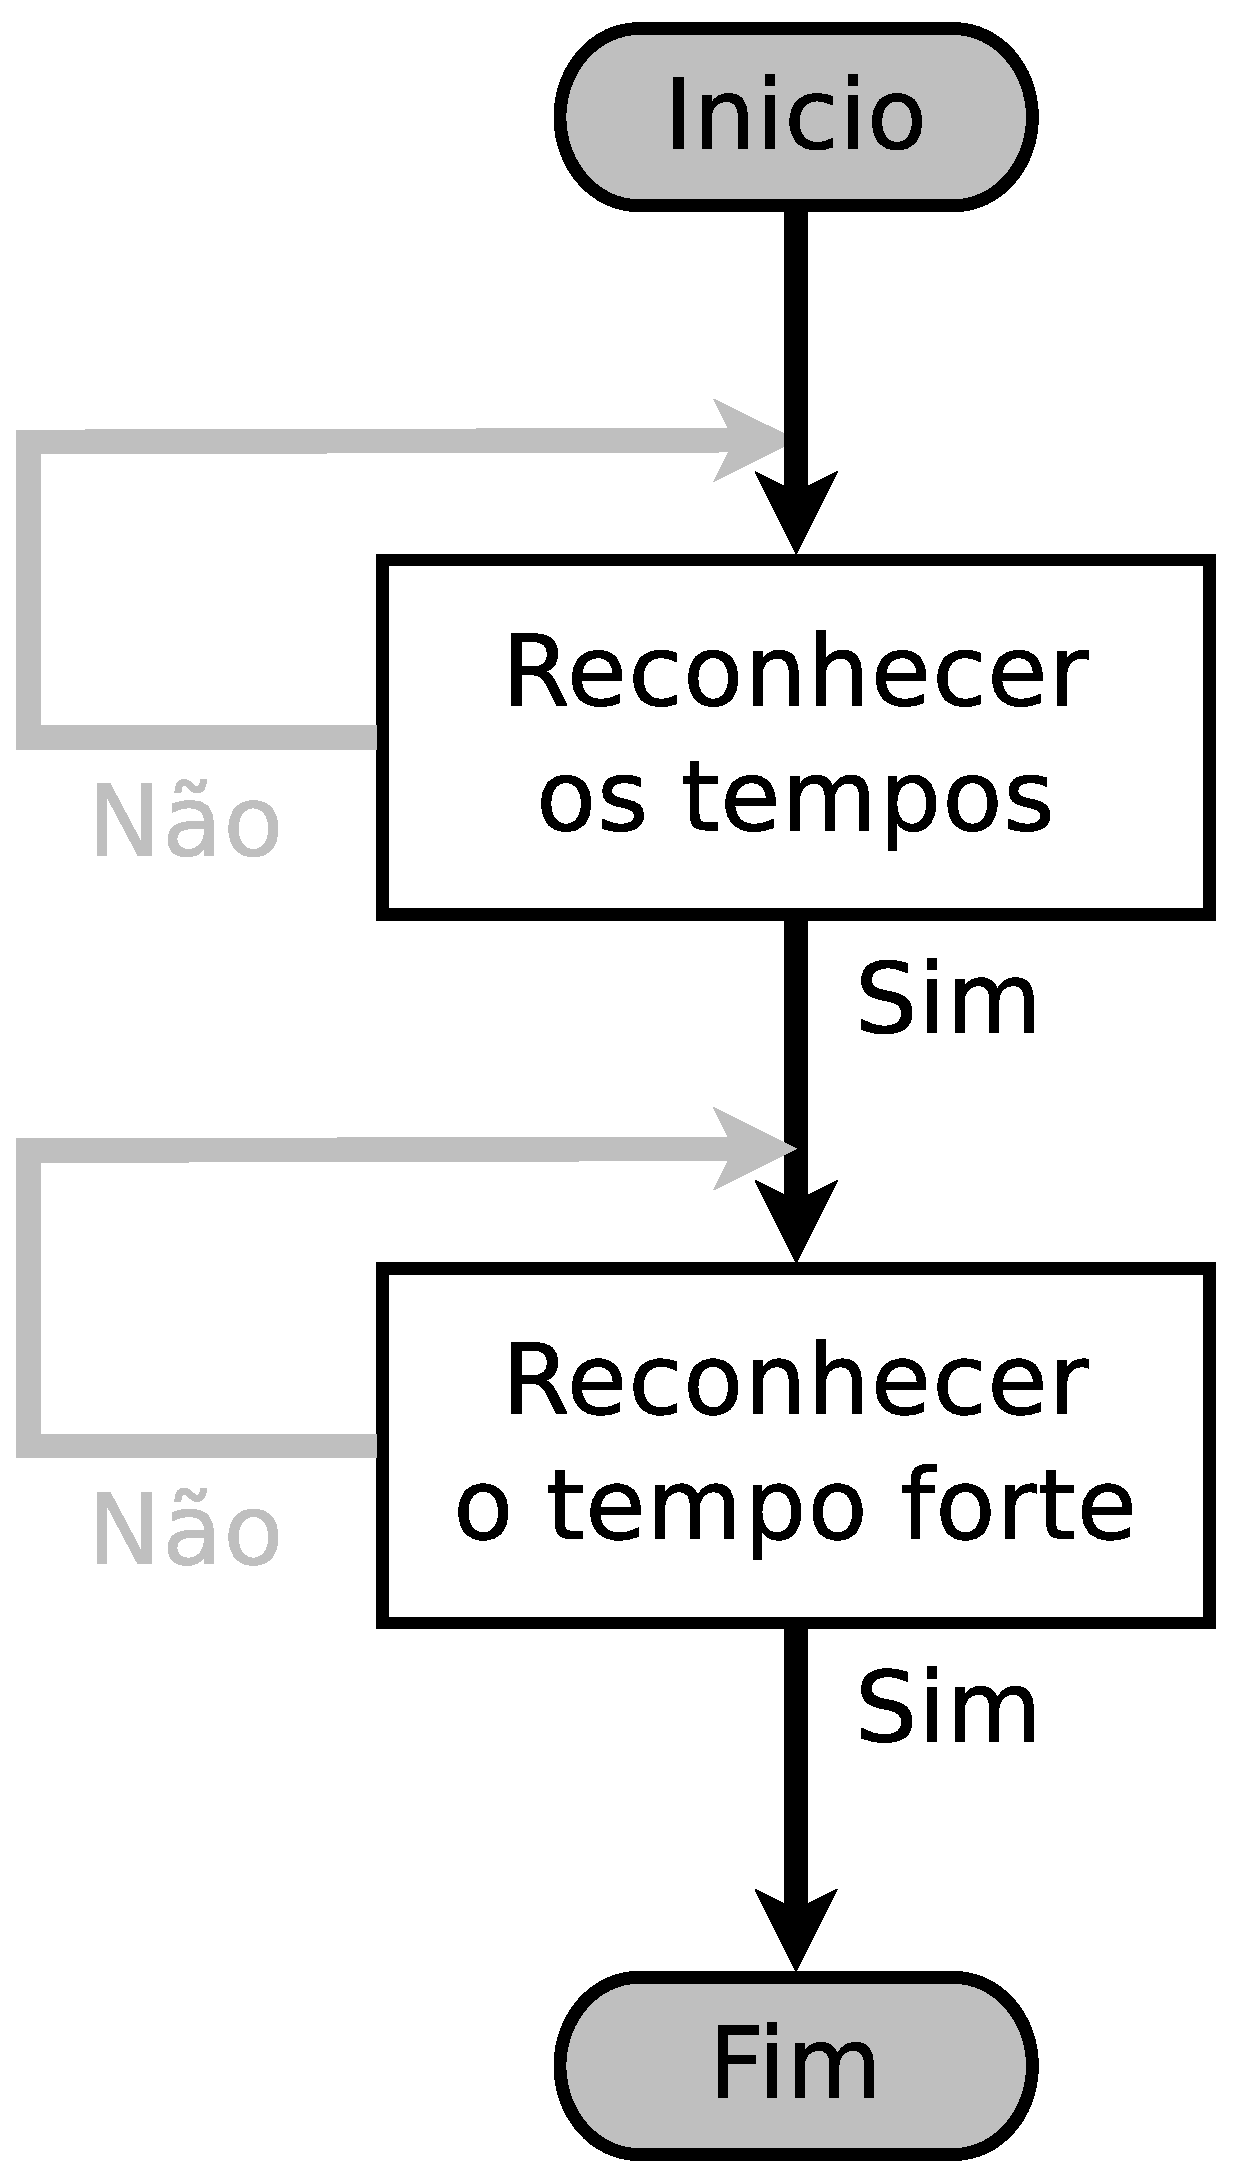
\includegraphics[width=0.65\textwidth]{chapters/cap-musicalidade-percepcion/dancanopulso2.eps}
\caption{Método quase-subjetivo}
\label{fig:fluxodancanopulso2}
\end{subfigure}
    \caption{Percebendo a métrica de uma música}\label{fig:fluxodancanopulso}
\end{figure}



%%%%%%%%%%%%%%%%%%%%%%%%%%%%%%%%%%%%%%%%%%%%%%%%%%%%%%%%%%%%%%%%%%%%%%%%%%%%%%%%
\subsection{Reconhecer o pulso}
\index{Musicalidade!Percepção do pulso}
\label{subsec:perpulsomusica}
As pessoas tendemos a dar palmas ou pisar com o pé, para acompanhar o ritmo da música como um todo,
isto acontece porque inconscientemente percebemos nela um batimento,
continuo e regular, como os batimentos do coração;
assim, quando damos palmas para acompanhar à música, o que estamos 
fazendo e reconhecer o  \hyperref[ref:Pulso]{\textbf{pulso}} musical. 

Este ato está vinculado mais a uma sensação que a um raciocínio,
pelo que é difícil apontar um método para reconhecer o pulso,
que não seja simplesmente indicar que debemos bater palmas ate ``sentir'',
que o pulso das palmas acompanhe ao pulso da música\footnote{Uma
sugestão é fazer isto fechando os olhos para evitar distrações e agudizar os outros sentidos. }.

Porém, sim podemos apontar alguns motivos que inconscientemente nos provocam chegar a este estado de sincronia.
Por exemplo, na Figura \ref{ritmo:procurando-pulso1},
\begin{figure}[!h]
\centering
    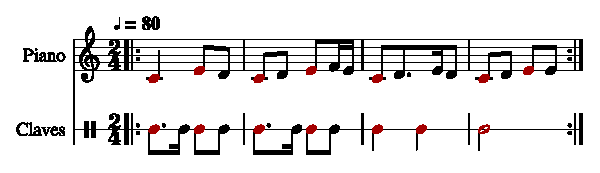
\includegraphics[width=\textwidth]{chapters/cap-musicalidade-percepcion/procurando-pulso1-1.eps}
\caption{Melodia e percussão.}
\label{ritmo:procurando-pulso1}
\end{figure}
podemos ver uma melodia acompanhada por uma percussão,
sendo ``piano'' e ``claves'' escritas usando  \hyperref[subsec:compassobinario]{\textbf{compassos binários}}, 
é dizer com dois tempos, um forte e um fraco, equivalentes cada um à duração de um \hyperref[ref:Pulso]{\textbf{pulso}}.
Assim, se nós fazemos a experiencia de escutar a música descrita na Figura \ref{ritmo:procurando-pulso1},
``sentiremos'' que podemos dar palmas ate sincroniza-nos com o pulso da música\footnote{Oito
palmas em total ate que a música seja reiniciada.}.
Isto é possível, 
a pesar de que em ambos casos as \hyperref[sec:figurasmusicais]{\textbf{figuras musicais}} usadas tem na sua maioria
\hyperref[sec:pos:Duracion]{\textbf{durações}} menores a um tempo;
podemos ver também o uso em menor quantidade de figuras musicais de um tempo de duração,
e só uma vez (no quarto compasso das claves) o uso de uma figura musical maior a um tempo. 
Pelo que podemos afirmar que em media as figuras musicais são menores a um tempo ou um pulso; consequentemente, 
não é esta a informação que usamos inconscientemente para achar o pulso,
devido a que é menor;
mas sim nos dá uma  aproximação do \hyperref[sec:Andamento]{\textbf{andamento}} da música,
aproximação que corrigirmos quando achemos o pulso.
Mas, existem informações que não são perdidas quando usamos figuras musicais menores ou maiores a um pulso,
e estas  são: o \hyperref[def:acentometrico]{\textbf{acento métrico}} e a 
distribuição de \hyperref[eq:acentosubdividio]{\textbf{acentos nas subdivisões de tempos}},
descrita na Pag. \pageref{eq:acentosubdividio}.
Assim, quando uma figura musical  é executada numa subdivisão do tempo, 
esta terá um acento proporcional a esta subdivisão;
por exemplo, uma figura executada na parte fraca do tempo fraco\footnote{Como
a terceira figura musical, do primeiro compasso do piano.}, 
terá um acento menor que uma executada num tempo fraco\footnote{Como
a segunda figura musical, do primeiro compasso do piano.}, 
e uma figura musical executada num tempo fraco terá um acento menor que a de um tempo forte\footnote{Como
a primeira figura musical, do primeiro compasso do piano.}.
Pelo que se deduz, que o que detetamos quando sentimos o pulso, 
é esse fluxo de \hyperref[sec:pos:Intensidade]{\textbf{intensidades}} mudando no tempo, 
como pode ser visto na Figura \ref{ritmo:procurando-pulso2}.
\begin{figure}[!h]
\centering
    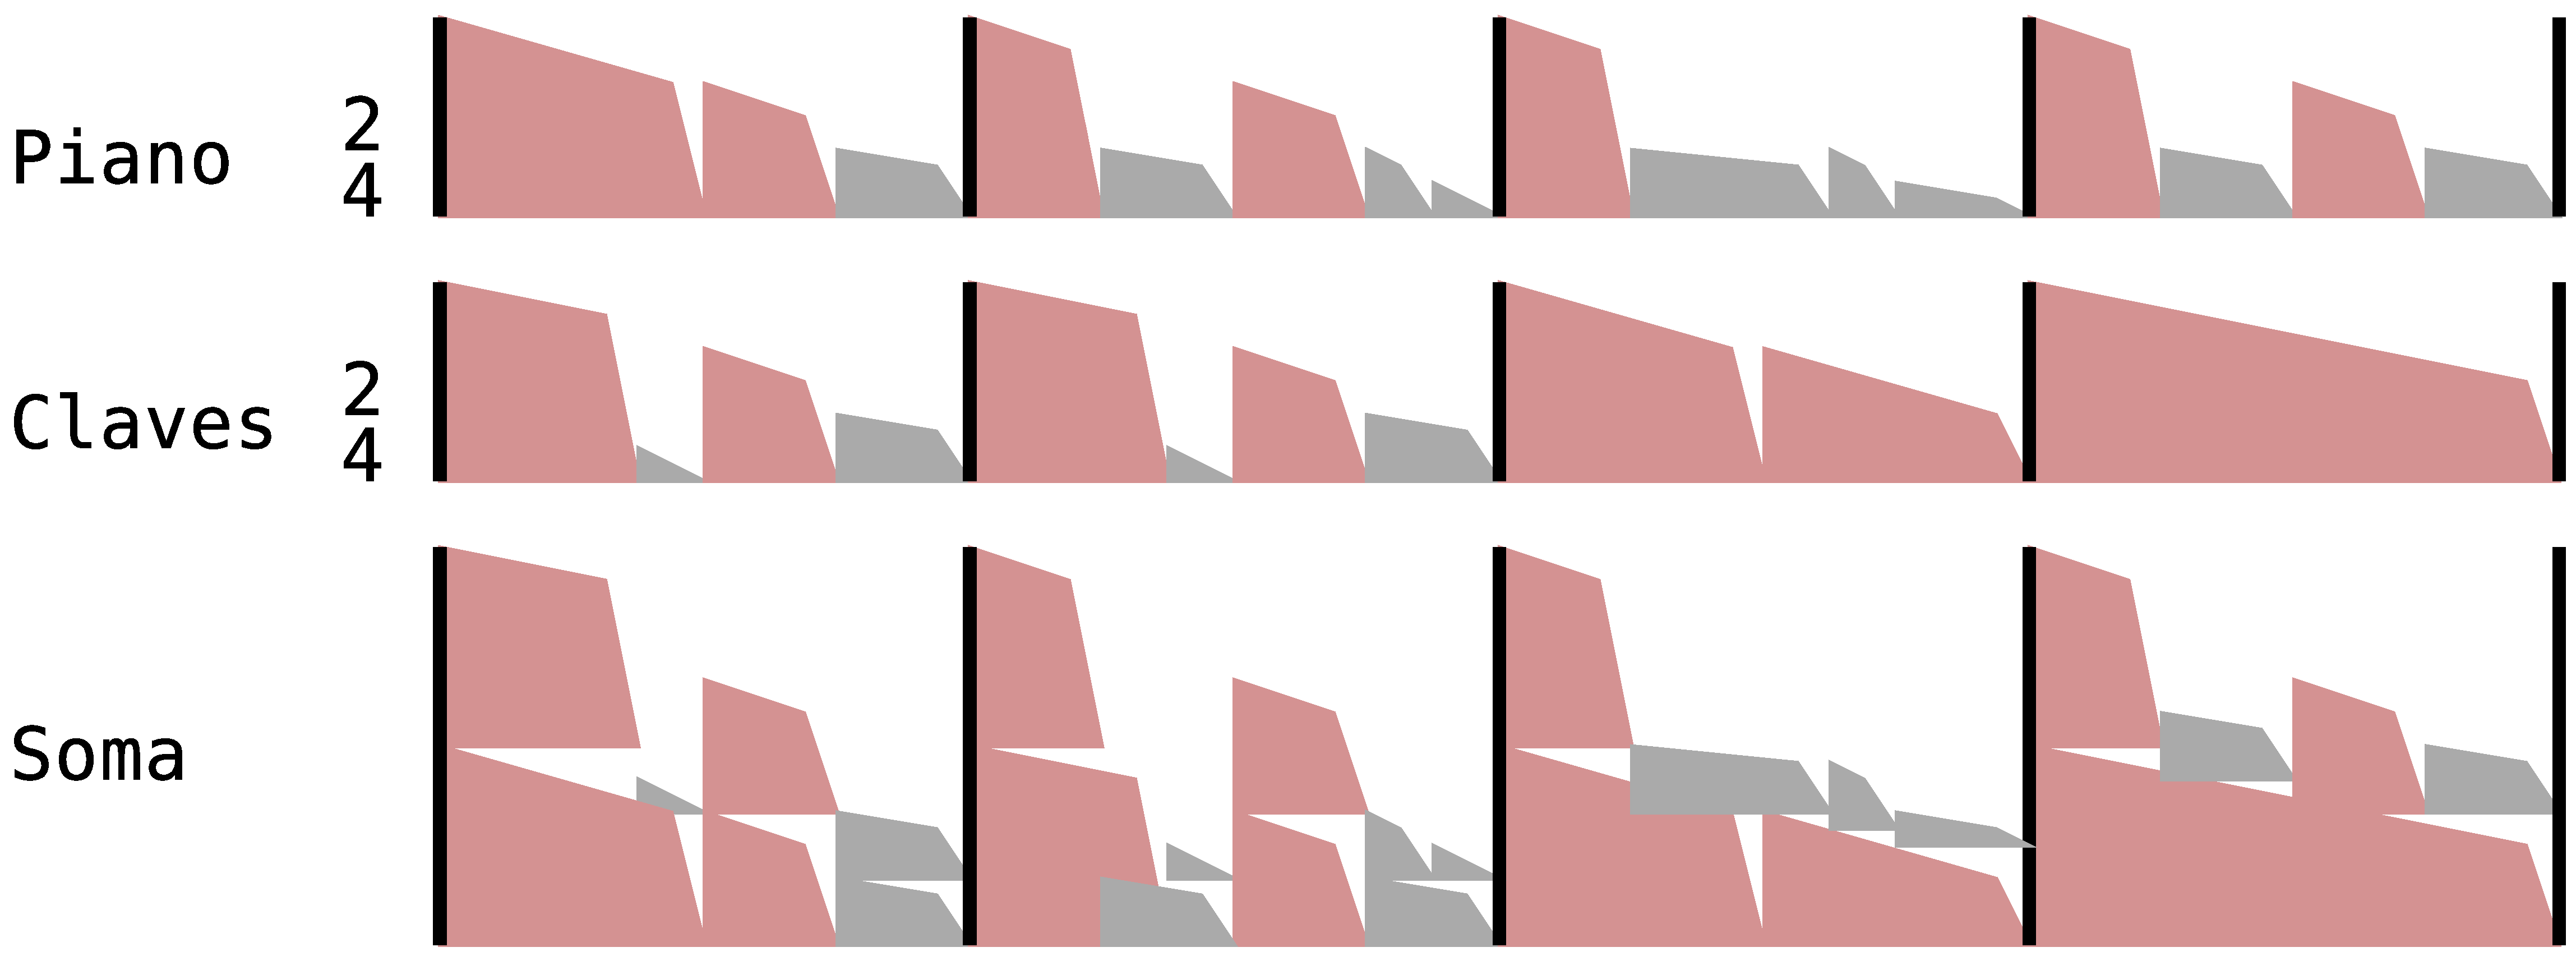
\includegraphics[width=\textwidth]{chapters/cap-musicalidade-percepcion/procurando-pulso2.eps}
\caption{Intensidades na melodia e percussão.}
\label{ritmo:procurando-pulso2}
\end{figure}
Onde temos uma aproximação do diagrama de intensidades: do piano, da clave e da soma de ambos;
no diagrama da ``soma'' fica mais claro porquê inconscientemente detetamos o fluxo de acentos,
e poderíamos inferir que este fluxo ficaria mais próximo ao fluxo do pulso, 
quando aumente o número de instrumentos envolvidos.


%%%%%%%%%%%%%%%%%%%%%%%%%%%%%%%%%%%%%%%%%%%%%%%%%%%%%%%%%%%%%%%%%%%%%%%%%%%%%%%%
\subsection{Reconhecer o tempo forte}
\index{Musicalidade!Tempo forte}
\index{Musicalidade!Bússola}
\label{subsec:perceberTF1}

\begin{wrapfigure}{r}{0.2\textwidth}
  \vspace{-10pt}
  \centering
    \includegraphics[width=0.15\textwidth]{compass.eps}
  \vspace{-10pt}
\end{wrapfigure}
O tempo forte é o primeiro tempo de cada \hyperref[def:Compasso]{\textbf{compasso}},
este nos ajudará a orientar-nos (bússola) em referencia à métrica da música, 
se precisamos identificá-lo numa música, podemos usar as seguintes informações:
\begin{itemize}
\item O tempo forte é o tempo em que estatisticamente percebemos que as vozes e 
instrumentos convergem executando as notas musicais com maior  \hyperref[sec:pos:Intensidade]{\textbf{intensidade}}  (potencia sonora). 
\end{itemize}

\begin{itemize}
\item Os compositores, seguindo a \hyperref[sec:ProsodiaMusical]{\textbf{prosódia musical}} vista Seção \ref{sec:ProsodiaMusical}, 
geralmente colocam as sílabas tônicas, das palavras, no tempo forte da música  \cite[pp. 149]{medteoria}. 
Da mesma forma, se fazemos um esforço de imaginação e pensamos que os instrumentos ``falam'' ou ``cantam chorando'',
podemos perceber o tempo forte identificando quê ``sílabas'' tem maior intensidade.
\item Se numa música pertencente a alguns dos \hyperref[sec:FamiliaSamba]{\textbf{subgeneros do samba}}, 
conseguimos identificar audivelmente  um padrão de repetição com a onomatopeia ``tchic-tchic tum'', 
então o tum é executado no tempo forte. 
Para mais detalhes ir a Seção \ref{sec:percepcaosamba1}.
\end{itemize}~

Lembremos que esta será uma procura do tempo forte por uma aproximação estatística, 
pois os acentos na música além de estar no tempo forte, 
também aparecem em tempos fracos, nos \hyperref[sec:contratempo]{\textbf{contratempos}}.




Além das indicações anteriores, 
existem outros critérios um pouco mais elaborados para conseguir identificar o tempo forte:
\begin{itemize}
\item Se percebemos um breque (break) na música, 
provocado por uma \hyperref[sec:Frase]{\textbf{frase}} com \hyperref[subsec:FinalAbertoFechado]{\textbf{final fechado}} 
(satisfatório, com uma sensação de ponto final), então este aconteceu no tempo forte.
\item A frase rítmica, das vozes que geram o acompanhamento da melodia principal,
geralmente iniciam no tempo forte; 
o inicio da frase é percebido com uma nota em tempo forte com maior intensidade, 
que a percebida em um tempo forte qualquer\footnote{Pode ser
devido a que se imprime de fato maior intensidade o a que mais instrumentos convergem nesse instante.}.
\end{itemize}

\begin{tcbattention}
É importante ressaltar que na música, 
a melodia principal acentua regularmente seguindo a \hyperref[def:acentometrico]{\textbf{métrica}}
e enfeita acentuando esporadicamente em \hyperref[sec:contratempo]{\textbf{contratempo}}.
Já o acompanhamento percussivo ou harmônico, por sua caraterística regular no padrão do seu ritmo,
geralmente opta por tocar continuamente acentuando no tempo forte,
ou continuamente no contratempo; 
por exemplo na música do reggae o acompanhamento geralmente está a contratempo.
\begin{itemize}
\item ``No Woman No Cry'' de Bob Marley.
\end{itemize}
\end{tcbattention}



%%%%%%%%%%%%%%%%%%%%%%%%%%%%%%%%%%%%%%%%%%%%%%%%%%%%%%%%%%%%%%%%%%%%%%%%%%%%%%%%
\subsection{Reconhecer o tipo de compasso}
\index{Musicalidade!Percepção do tipo de compasso}
\label{subsec:pertipodecompasso}
Se já conseguimos \hyperref[subsec:perceberTF1]{\textbf{identificar o tempo forte}} na música,
então podemos dizer que conhecemos o ciclo de repetição imposto pela métrica,
e podemos predizer quando acontecerá o próximo tempo forte.
Tendo em conta tudo o anterior,
o seguinte passo é deduzir quantos tempos fracos acontecem 
entre um par consecutivo de tempos fortes;
é dizer, 
temos que identificar se a música tem compassos 
\hyperref[subsec:compassobinario]{\textbf{binários}} (2 tempos), 
\hyperref[subsec:compassoternario]{\textbf{ternários}} (3 tempos), 
\hyperref[subsec:compassoquaternario]{\textbf{quaternários}} (4 tempos) 
ou outros. 

Uma forma de deduzir o tipo de compasso utilizado na música  é usando como guia o estilo musical; por exemplo:
\begin{itemize}
\item As músicas dos \hyperref[sec:FamiliaSamba]{\textbf{subgêneros do samba}} 
são principalmente escritas em compassos binários,
porém também é possível ver o uso de compassos quaternários ou de compassos compostos.
\item As músicas de forró comumente usam compassos quaternários,
porém também é possível ver o uso de compassos binários, como no baião. 
\item Em músicas usadas para dançar bolero, salsa, zouk 
e sertanejo universitário é comum perceber o uso de compassos quaternários.
\item Nas músicas onde se dança valsa são usados compassos ternários. Etc.
\end{itemize}
Em geral a maioria da música popular ``de moda'', no \AnoLivro, usa uma quantidade par de tempos no compasso;
sendo quaternários em primeiro lugar e binários em segundo.
Pelo que se o estilo musical não é valsa (compassos ternários), 
teremos muito provavelmente um número par de tempos no compasso;
porém, é  pouco provável atualmente achar (na rádio ou em sites de música),
o destaque de músicas em ritmo de valsa.

O método que seguiremos para identificar o tipo de compasso será testar estes tipos,
um a um, ate perceber entre eles uma maior coincidência,
iniciando o teste com o tipo de compasso com mais probabilidade seguindo o estilo musical \cite[pp. 10]{wright1992social}.
Assim, testaremos primeiro os compassos (simples)
\hyperref[subsec:compassobinario]{\textbf{binários}}, 
\hyperref[subsec:compassoternario]{\textbf{ternários}}, 
\hyperref[subsec:compassoquaternario]{\textbf{quaternários}};
se for necessário testaremos alguns compassos compostos 
e em muitas raras ocasiões os compassos mistos.

Não precisamos testar a métrica com a música como um todo,
e sim podemos usar melodias ou ritmos de instrumentos isolados para testar a métrica \cite[pp. 10]{wright1992social};
por exemplo, no caso de musicas com \hyperref[subsec:homofonica]{\textbf{textura homofônica}},
geralmente pela natureza repetitiva e marcada do acompanhamento ou da percussão,
é mais fácil detetar a métrica nessas camadas da música.

\subsubsection{Testando um compasso binário}
A forma mais simples de detetar a métrica dos compassos \hyperref[subsec:compassobinario]{\textbf{binários}},
é fazendo uma troca de peso entre nossos pés (balanço),
ate encaixar o tempo forte\footnote{Para ter certeza de que detetamos o tempo forte, 
podemos usar as técnicas explicadas na Seção \ref{subsec:perceberTF1}.} 
de um lado de nosso balanço,
e perceber que a contagem binária bate com o \hyperref[ref:Pulso]{\textbf{pulso}} da música,
e com uma distribuição de acentos, \{Forte, fraco\};
nesse ponto deduziremos de quê lado do balanço está o tempo forte e o fraco.

\begin{example}[Música com compassos de 2 tempos:]
\label{ex:compassosimples3t}
A música ``Piston de Gafieira'' de Billy Blanco,
está composta por compassos binários (simples), pelo qual tem 2 tempos.
Um exercício interessante, é \hyperref[subsec:perceberTF1]{\textbf{achar o tempo forte}},
por exemplo seguindo as sílabas tônicas na letra da música,
e tentar encaixar a contagem:\{\textbf{1}, 2\}, no ciclo da métrica, acentuando cada tempo 1 (tempo forte). 
\end{example}

\begin{example}[Outros exemplos de compassos binários:]
~
\begin{itemize}
\item ``Tico-Tico no fubá'' de Zequinha de Abreu  \cite[pp. 6]{marcondes1998enciclopedia} \cite[pp. 39,91]{diniz2003almanaque}.
\item ``Brasileirinho'' de Valdir Azevedo  \cite[pp. 133]{perna2002samba}.
\item ``Pelo telefone'' de  Ernesto dos Santos (Donga) e Mauro de almeida.
\item ``Pierrô apaixonado'' de Heitor dos prazeres e Noel Rosa \cite[pp. 1070]{marcondes1977enciclopediav2} \cite[pp. 53]{diniz2008almanaque}.
\item ``A banda'' de Chico Buarque interpretada por Nara Leão \cite[pp. 90]{diniz2008almanaque} \cite{partituraabanda1}.
\end{itemize}
\end{example}


\subsubsection{Testando um compasso ternário}
Neste caso bastará que nós contemos ate 3, iniciando em 1 no tempo forte,
e procurando que os três tempos encaixem perfeito no ciclo da métrica (entre dois tempos fortes consecutivos).
Se percebemos que esta contagem encaixa na métrica,
com uma distribuição de acentos, \{Forte, fraco, fraco\} \cite[pp. 10]{wright1992social}, 
então estamos sim, frente a um  \hyperref[subsec:compassoternario]{\textbf{compasso ternário}}.

\begin{example}[Música com compassos de 3 tempos:]
\label{ex:compassosimples3t3}
A música ``João e Maria'' de Chico Buarque,
está composta por compassos ternários (simples), pelo qual tem 3 tempos.
Um exercício interessante, é \hyperref[subsec:perceberTF1]{\textbf{achar o tempo forte}},
por exemplo seguindo as sílabas tônicas na letra da música,
e tentar encaixar a sequencia:\{\textbf{1}, 2 , 3\}, no ciclo da métrica,acentuando cada tempo 1 (tempo forte). 
\end{example}

\begin{example}[Outros exemplos de compassos ternários:]
\label{ex:compassosimples3t2}
~
\begin{itemize}
\item ``Rio grande tchê'' interpretado pelo grupo Os serranos.
\item ``Blusa Vermelha'' interpretado pelo Trio Parada Dura.
%\item ``Ainda ontem chorei de saudade'' interpretado por Eduardo Costa e Leonardo.
\item ``Último adeus'' interpretado por Eduardo Costa e Leonardo.
\item ``Chao de Giz'' de Ze Ramalho.
\end{itemize}
\end{example}

\subsubsection{Testando um compasso quaternário}
Neste caso nos temos que contar ate 4, iniciando em 1 no tempo forte,
e procurando que os quatro tempos encaixem perfeito no ciclo da métrica.
Se percebemos que esta contagem encaixa na métrica (entre dois tempos fortes consecutivos),
com uma distribuição de acentos, \{Forte, fraco, meio forte, fraco\} \cite[pp. 10]{wright1992social}, 
então estamos sim, frente a um  \hyperref[subsec:compassoquaternario]{\textbf{compasso quaternário}}.


\begin{example}[Música com compassos de 4 tempos:]
\label{ex:compassosimples4t}
A música (\hyperref[subsec:marcha]{\textbf{Marcha}}) ``Noite dos Mascarados'' de Chico Buarque,
está composta por compassos quaternários (simples), pelo qual tem 4 tempos,
e podemos contar: \{\textbf{1}, 2 , 3, 4\}, acentuando cada tempo 1 (tempo forte) e cada tempo 3 (tempo semi forte).
Um exercício interessante, é \hyperref[subsec:perceberTF1]{\textbf{achar o tempo forte}},
por exemplo seguindo as sílabas tônicas na letra da música,
e tentar encaixar a sequencia da contagem no ciclo da métrica, 
\end{example}

\begin{example}[Outros exemplos de compasso quaternário:]
~
\begin{itemize}
\item ``Sambolero'' interpretado por Luiz Bonfá \cite[pp. 49]{sambolero}.
\item ``Cê que sabe'' interpretado por Cristiano Araujo.
\item ``Vai dar namoro'' interpretado por Bruno e Marrone.
\item ``Vou te amarrar a minha cama'' interpretado por Bruno e Marrone.
\item ``Borbulhas de amor'' interpretado por Eduardo costa e Leonardo%Gustavo Lima.
\end{itemize}
\end{example}

\subsubsection{Compassos compostos}
Na prática, bastará a principio, para um dançarino iniciante,
reconhecer os compassos \hyperref[subsec:compassoquaternario]{\textbf{quaternários}}, 
\hyperref[subsec:compassobinario]{\textbf{binários}}, e 
\hyperref[subsec:compassoternario]{\textbf{ternários}},
nesse ordem de ocorrência;
pois as raras ocasiões onde estejamos frente a um \hyperref[sec:compaso]{\textbf{compasso composto}},
um dançarino pode tratar ele como sua contraparte simples,
e desenvolver-se suficientemente bem na dança. 
Podemos perceber o uso de compassos compostos de 6 pulsos nos Exemplos \ref{ex:compassocomposto6}
e \ref{ex:compassocomposto6b},
este tipo de compassos é muito comum nas baladas pop e na música erudita.
\begin{example}[Música com compassos de 6 pulsos:]
\label{ex:compassocomposto6}
Um exemplo deste tipo de música pode ser escutado em ``A Thousand Years'', 
interpretado por Christina Perri. É fácil perceber como podemos nos confundir,
pensando que a música usa compassos binários (simples) de andamento lento,
ou ternários de andamento rápido; quando na realidade trata-se de compassos binários compostos de 6 pulsos (dois tempos),
possivelmente com formula de compasso 6/8.

Um dançarino, mesmo sabendo que trata-se de um \hyperref[compasso:binario]{\textbf{compasso binário composto}} (de 6 pulsos),
pode tratar a música como se esta fosse binária simples, e dançar em grupos de dois passos lentos,
ou como se fosse ternaria simples, e tentar dançar estilo valsa porém muito rápida.

A mínima subdivisão a ser feita por nós na dança, 
será a de assumir um compasso binário, usando movimentos binários,
pois quando tentemos subdividir por dois um passo, para encaixar um ``tchic tchic tum'',
acharemos a dança desconfortável, devido a que
entraremos em conflito com o \hyperref[ref:Pulso]{\textbf{pulso}}, 
que divide o compasso em porções múltiplos de três.
  
\end{example}

\begin{example}[Outros exemplos de compassos binários de 6 pulsos:]
\label{ex:compassocomposto6b}
~
\begin{itemize}
\item ``Quem é ela'' interpretado por Marco e Mário.
\item ``Seu amor ainda é tudo'' interpretado por Eduardo Costa e Leonardo.
\item ``You don't own me'' interpretado por Grace.
\item ``We are the champions'' interpretado pelo grupo Queen.
\item ``Hallelujah'' interpretado por Rufus Wainwright.
\item ``Happy Christmas'' interpretado por John Lennon.
\item ``The House of the Rising Sun'' interpretado pelo grupo  The Animals.
%\item ``Lakmé'' interpretado por Léo Délibes.
%\item ``Nothing Else Matters'' interpretado pelo grupo Metallica.
\end{itemize}
\end{example}

\subsubsection{Compassos mistos}
Em muitas raras ocasiões, mais raro ainda que o caso dos compassos compostos, 
podemos achar compassos mistos, como nos Exemplos \ref{ex:compassomisto5} e \ref{ex:compassomisto7}.

\begin{example}[Música com compassos de 5 pulsos:]
\label{ex:compassomisto5}
A música ``Take Five'' interpretada por  Dave Brubeck,
está composta por compassos mistos (alternados), criados pela concatenação de um compasso binário e um ternário,
contando-se os tempos: \{\textbf{1}, 2, \textbf{1}, 2, 3\}, acentuando o 1.
Um exercício interessante, é achar o tempo forte  e tentar encaixar esta sequencia na música, 
\end{example}

\begin{example}[Música com compassos de 7 pulsos:]
\label{ex:compassomisto7}
A música ``Money'' interpretada pela banda  Pink Floyd,
esta composta por compassos mistos (alternados), criados pela concatenação de um compasso quaternário e um ternário,
contando-se os tempos: \{\textbf{1}, 2 , 3, 4, \textbf{1}, 2, 3\}, acentuando cada tempo 1 e o primeiro 3 (meio forte).
Um exercício interessante, é achar o tempo forte  e tentar encaixar esta sequencia na música, 
\end{example}

%%%%%%%%%%%%%%%%%%%%%%%%%%%%%%%%%%%%%%%%%%%%%%%%%%%%%%%%%%%%%%%%%%%%%%%%%%%%%%%%
%%%%%%%%%%%%%%%%%%%%%%%%%%%%%%%%%%%%%%%%%%%%%%%%%%%%%%%%%%%%%%%%%%%%%%%%%%%%%%%%
\section{Percepção da métrica no samba}
\index{Musicalidade!Métrica no samba}
\label{sec:percepcaosamba1}

As músicas dos subgêneros do samba, as quais usamos para dançar, 
geralmente são escritas usando \hyperref[subsec:compassobinario]{\textbf{compassos binários}};
por este motivo a procura da métrica das músicas nesses subgêneros 
é mais simples, 
pois iniciamos a busca tendo a quase certeza do tipo do compasso, 
pelo que só precisaríamos \hyperref[subsec:perceberTF1]{\textbf{achar o tempo forte}} 
usando as indicações descritas na seção \ref{subsec:perceberTF1}.

Assim, para detetar o tempo forte e as \hyperref[sec:pos:Duracion]{\textbf{durações}} dos tempos nos compassos,
devemos ter em conta que quando escutamos uma música 
na qual é tipicamente dançado o samba, ou especificamente o samba de gafieira,
podemos distinguir que a união dos sons produzidos pelos instrumentos de percussão\footnote{Ou o
acompanhamento em geral.} 
geram um padrão de repetição muito particular, 
geralmente relacionado com as onomatopeias: ``tchic tchic tum'' ou ``tum tum''; 
em ambos  casos existe um  ``tum'' executado com maior 
\hyperref[sec:pos:Intensidade]{\textbf{intensidade}} (potencia sonora) e
que está sendo executado no tempo forte.
Se conseguimos detetar ou encaixar alguma destas duas onomatopeias na música,
então temos o problema resolvido, pois ambas ocupam exatamente dois tempos 
e dado que para conseguir encaixar as onomatopeias tivemos que reconhecer o tempo forte no ``tum'',
temos todos os elementos para descrever a métrica dos compassos na música.

\PRLsep{Analisando a música no samba}

A Figura \ref{fig:abc-caquarela} representa os compassos 18, 19 e 20 da  
composição musical ``Aquarela do Brasil'' escrita
por Ary Barroso em 1939 \cite{AquarelaDoBrasil}; 
a versão mostrada na figura teve arranjos por Irineu Krüger \cite{Irineu}.\\ 


\begin{figure}[ht]
\centering
\href{https://drive.google.com/file/d/1RcUcWJlukxaF7nmDTKDxUZDR8sLH9QpC/view?usp=sharing}{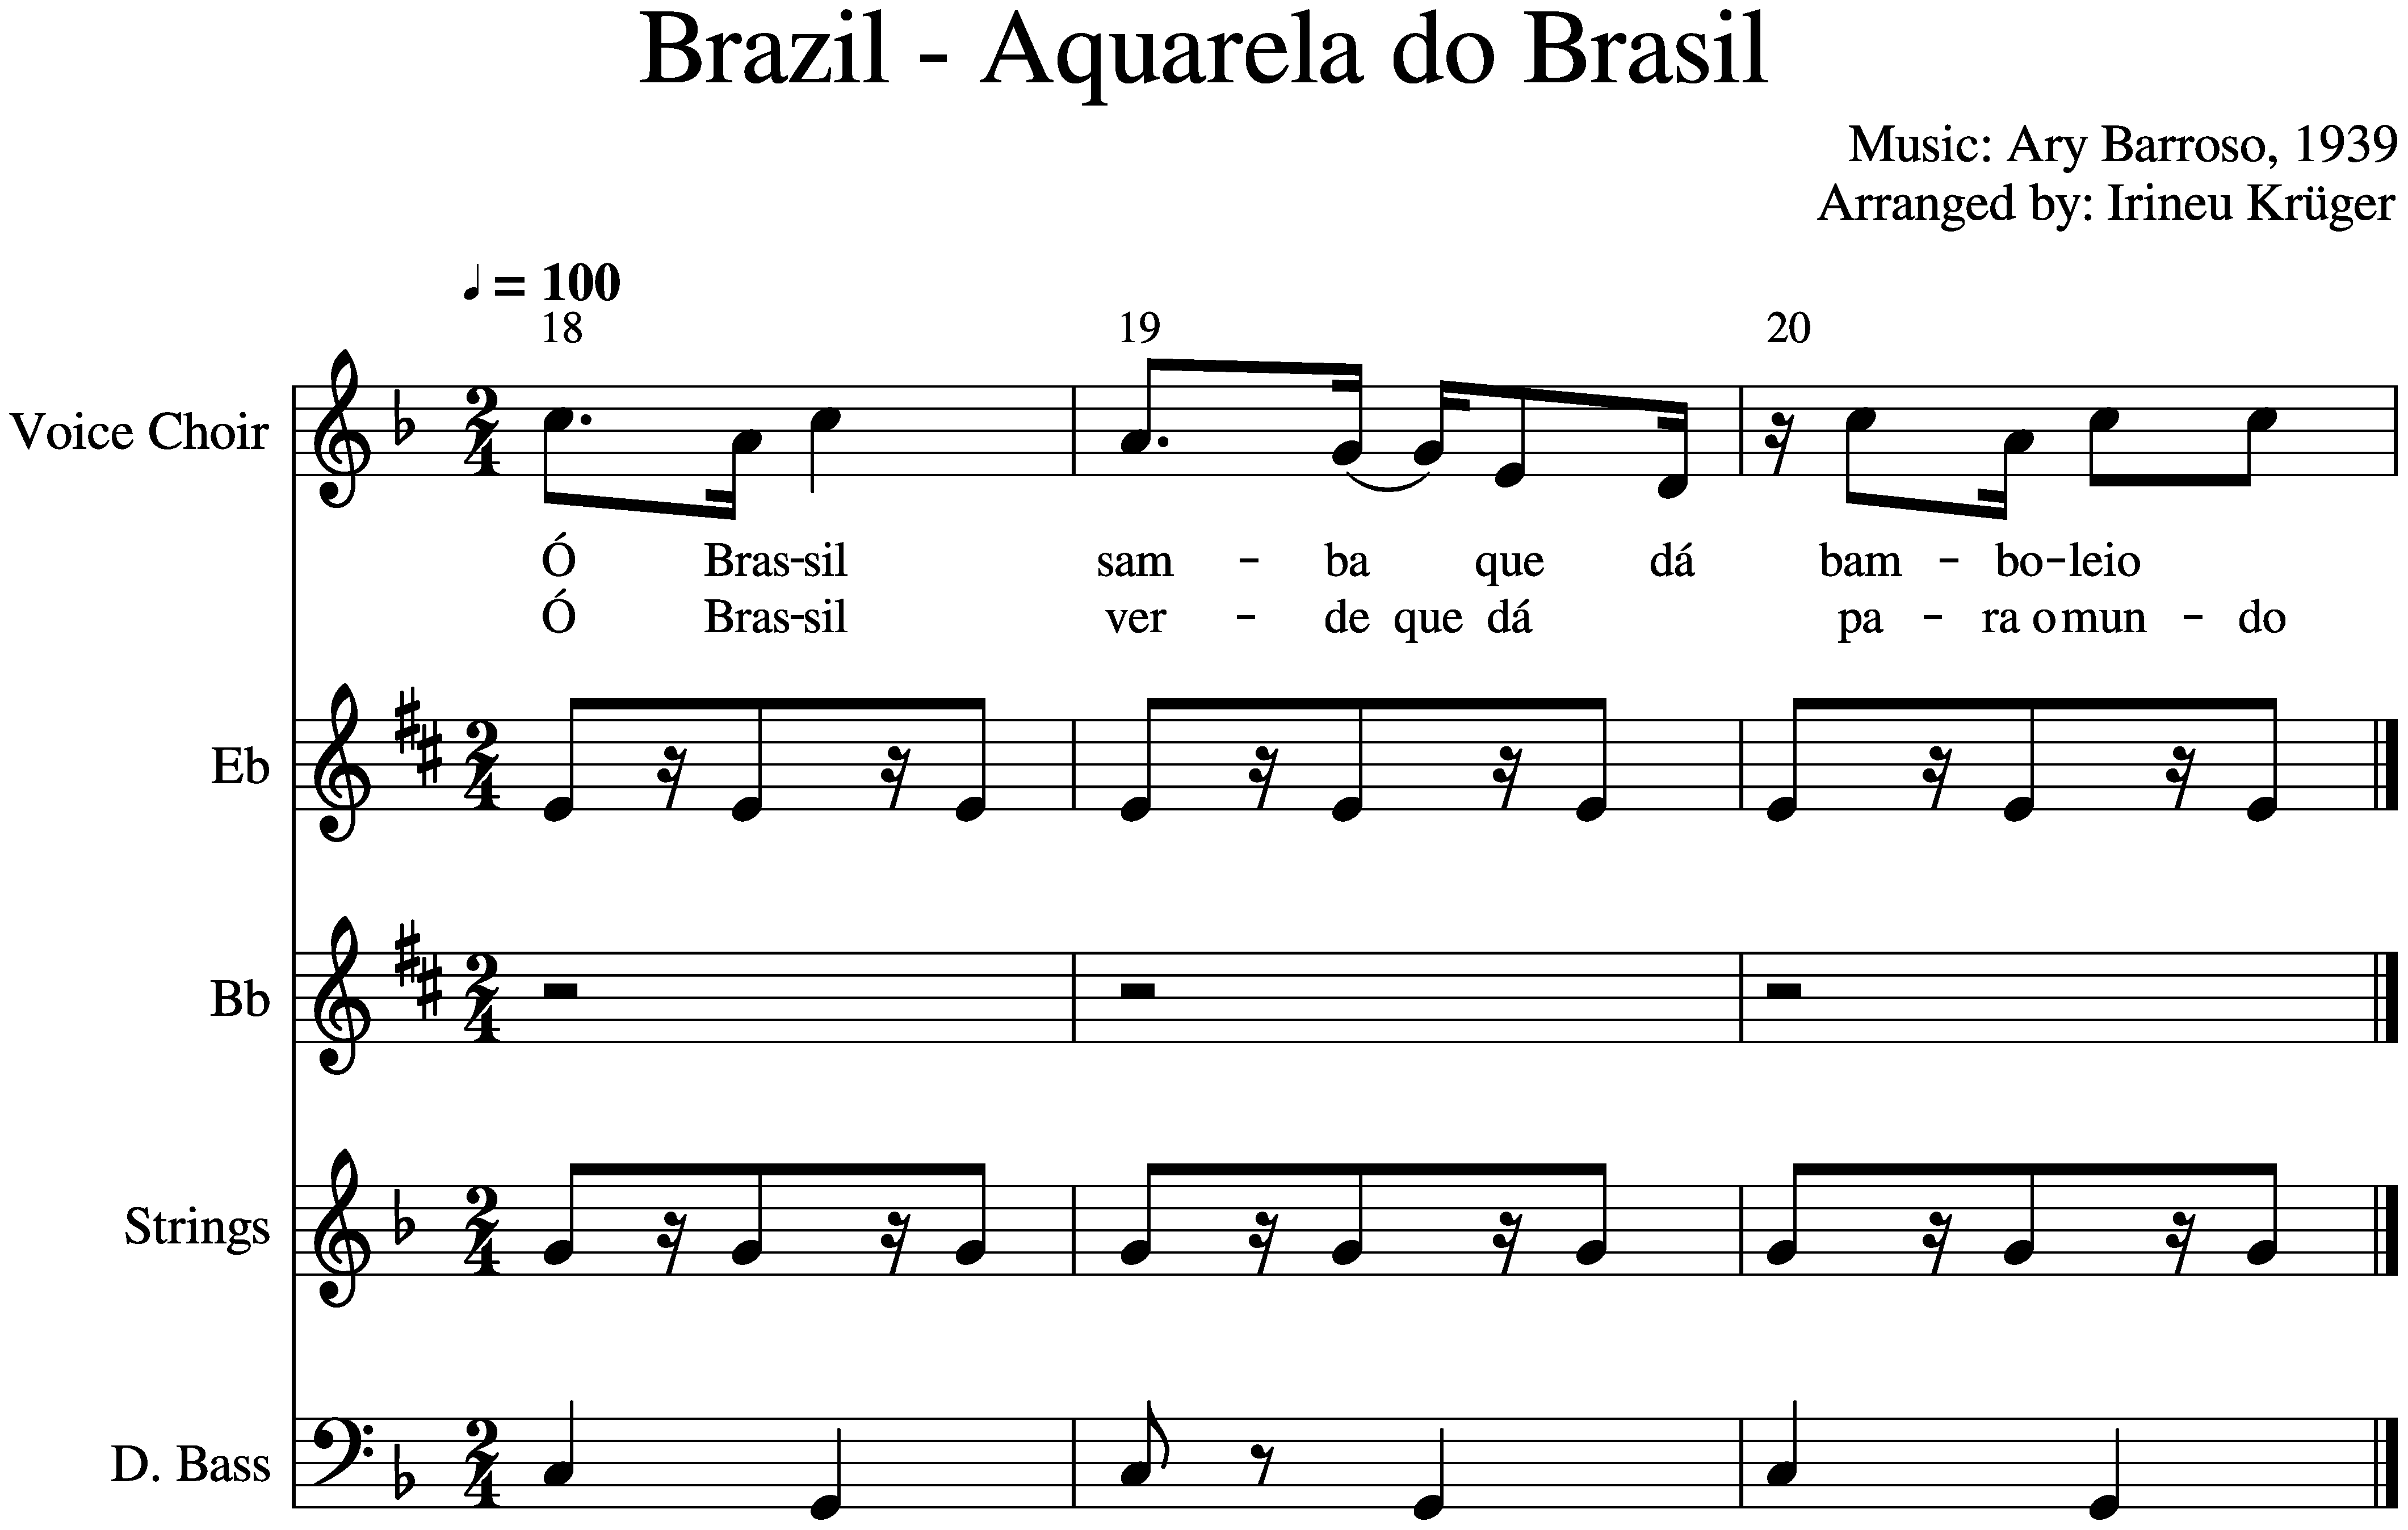
\includegraphics[width=0.99\textwidth]{chapters/cap-musicalidade-percepcion/abc-aquarela-1.eps}}
\begin{comment}
\begin{abc}[name=abc-caquarela]%,options={-O= -c -s 0.8}]
% abcm2ps aquarela.abc  -O aquarela.ps
% ps2epsi aquarela.ps aquarela.eps
%
X: 1 % start of header
T: Brazil - Aquarela do Brasil
C: Music: Ary Barroso, 1939
C: Arranged by: Irineu Krüger
K: Dm % scale: C major
Q:1/4=100
M: 2/4 % formula do compasso
%
V:1 clef=treble name="Voice Choir" sname="Voice Choir"
V:2 clef=treble name="Eb" sname="Eb"
V:3 clef=treble name="Bb" sname="Bb"
V:4 clef=treble name="Strings" sname="Strings"
V:5 clef=bass   name="D. Bass" sname=""D. Bass"
%
%
[V:1] "18" C'3/2A/2C'2  |"19" A3/2(G/2 G/2)E1D/2  |"20" z/2 C'1A/2 C'1C'1  |
w:    Ó Bras-sil        sam-ba_ que dá       bam-bo-leio_ 
w:    Ó Bras-sil        ver-de que dá_       pa-ra~o mun-do 
%
%
[V:2] [K:D] E1z/2E1z/2E1  | E1z/2E1z/2E1  | E1z/2E1z/2E1  |
%
%
[V:3] [K:D] z4  | z4  | z4  |
%
%
[V:4] [K:Dm] G1z/2G1z/2G1  | G1z/2G1z/2G1  | G1z/2G1z/2G1  |
%
%
[V:5] C,2 G,,2  | C,1 z1 G,,2  | C,2 G,,2  |
\end{abc}
\end{comment}
\caption{3 compassos da partitura da composição ``Aquarela do brasil''.}
\label{fig:abc-caquarela}
\end{figure}

Nesta versão, a música está escrita seguindo uma 
\hyperref[subsec:homofonica]{\textbf{textura homofônica}} com:
\begin{itemize}
\item \textbf{melodia principal:} 1 voz ou coro de voces (``Voice Choir'') e  
\item \textbf{acompanhamento:} 4 instrumentos (``Eb'',``Bb'',``Strings'' e ``D. Bass''), 
\end{itemize}
que usam uma 
formula de compasso $2/4$, de modo que se tem compassos
binários com tempos com uma \hyperref[sec:pos:Duracion]{\textbf{duração}} de uma semínima (\quarternote).


\begin{figure}[hb!]
\begin{elaboracion}{Jaime Arôxa e o ``tic tic tum''}
\index{Musicalidade!Tic tic tum}
\begin{wrapfigure}{r}{0.35\textwidth}
\centering
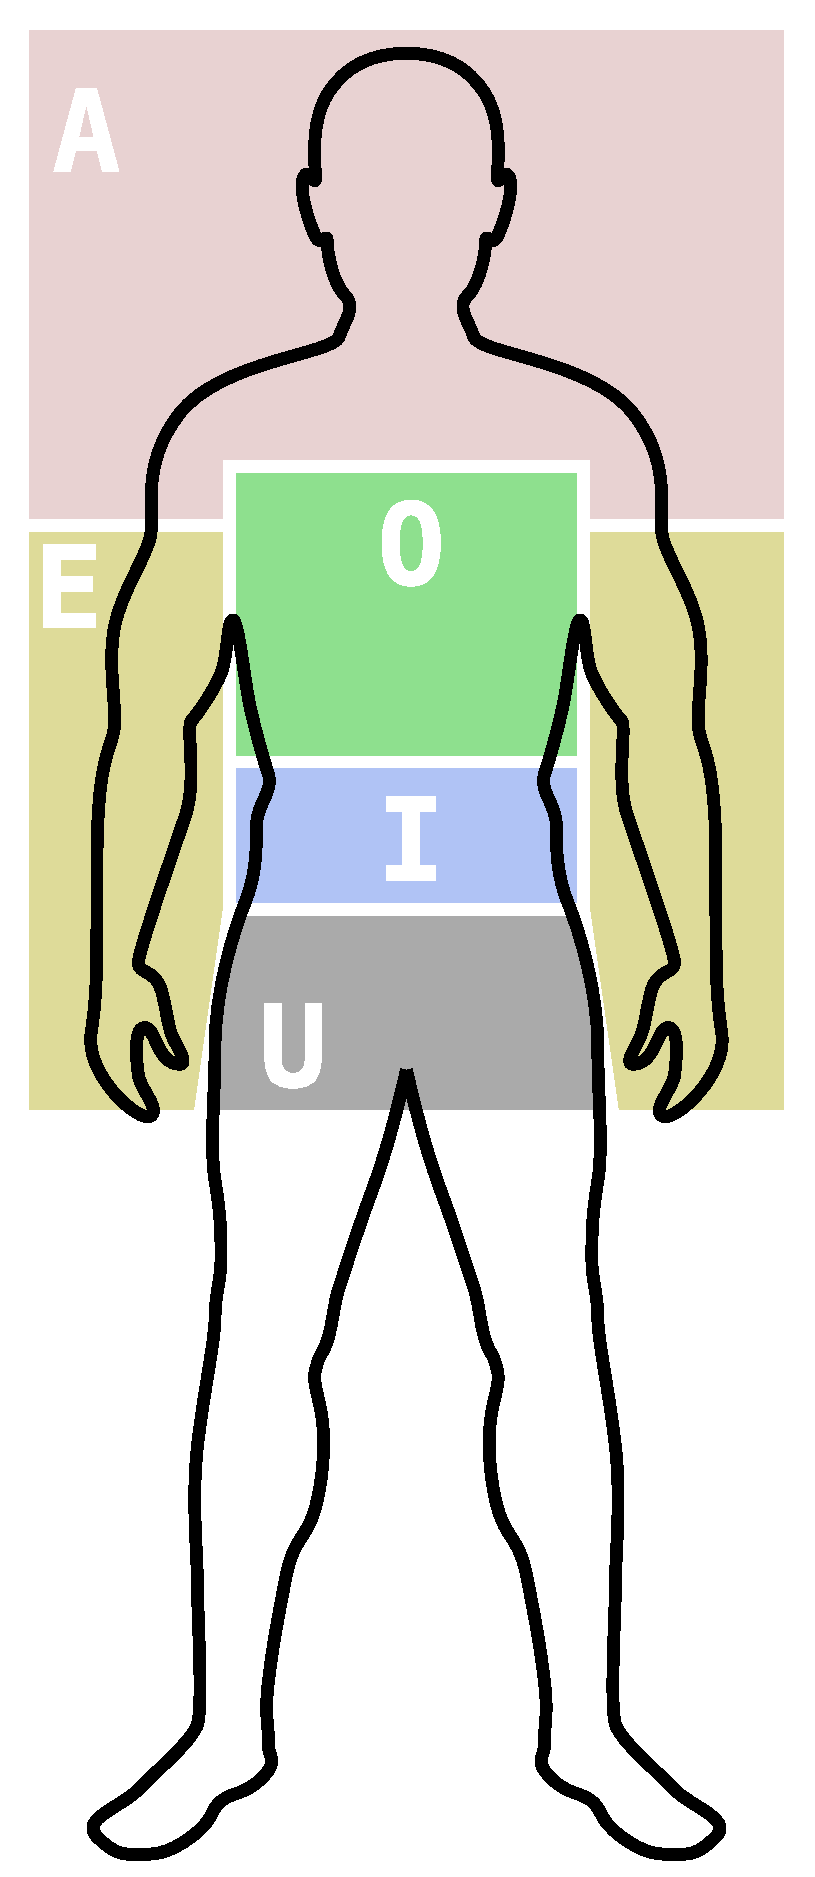
\includegraphics[width=0.33\textwidth]{chapters/cap-musicalidade-percepcion/aroxa-tic-tic-tum.eps}
\end{wrapfigure}
O renomeado professor de dança, coreografo e  dançarino, Jaime Arôxa \cite{JaimeAroxaSite},
numa de suas múltiplas contribuições ao ensino da dança de salão no Brasil,
criou ao redor do ano de 1991, 
o uso do ``tic tic tum''
\footnote{Popularmente também pode se achar o termo ``tchic tchic tum'' que tem só um sentido temporal, 
e não corporal como na didática proposta por Jaime.} 
para o ensino do ritmo nas aulas de samba de gafieira \cite{EntrevistaJaimeAroxa1};
numa tentativa de aproximar conceitos musicais a pessoas não iniciadas em música;
de modo que ele, na sua didática, não usava números e sim sons que eram fáceis de lembrar e interpretar.
Na sua proposta pedagógica, 
Jaime indica que cada parte do corpo pode estar atrelada a uma vogal.
\begin{description} 
\item[A:] Cabeça e ombros. 
\item[E:] Braços e mãos. 
\item[I:] Umbigo.
\item[O:] Embaixo dos ombros e o peito.
\item[U:] Bacia.
\end{description}
Assim, mecanicamente falando, o ``tic tic tum'' é ideal para o ensino do samba de gafieira
\footnote{Jaime ao redor do ano de 1991 criou o uso de ``tum e tum'' para bolero;
e em anos posteriores ``tum tum pá'' para o ensino de zouk.},
pois:
\begin{itemize} 
\item o ``tic'' está relacionado com uma contração do umbigo para deixar as pernas mais soltas;
\item o ``tum'' indica uma transferência total do peso do corpo pela ação da bacia;
\end{itemize}


Por outro lado, falando temporalmente, um ``tic tic tum'' descreve um ritmo com uma distribuição de tempos, 
no qual um ``tic'' dura a metade de tempo que um ``tum''. 
Uma forma de representar isto na notação musical pode ser vista na seguinte pauta.\\

\centering
\href{https://drive.google.com/file/d/1CZaAP5lPzVX7oTT5EMpIKN-XbOUYUt3Y/view?usp=sharing}{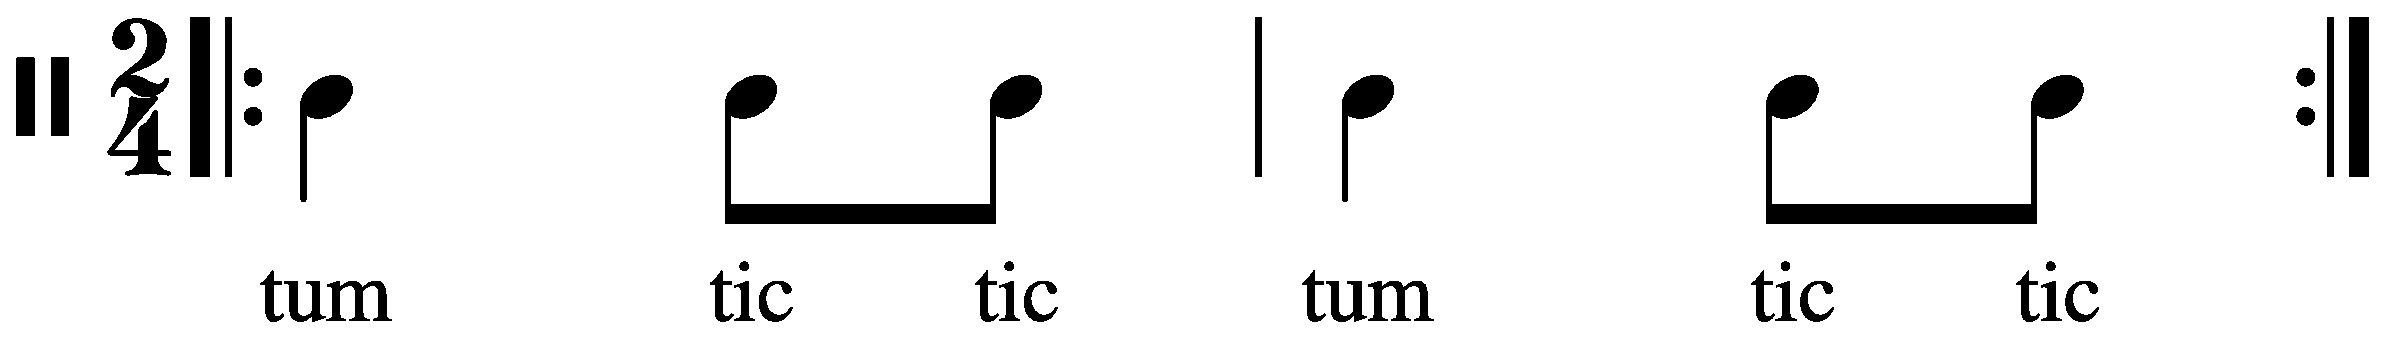
\includegraphics[width=0.7\textwidth]{chapters/cap-musicalidade-percepcion/abc-tictictumaroxa-1.eps}}
\begin{comment}
\begin{abc}[name=abc-tictictumaroxa,width=0.60\linewidth]
X: 1 % start of header
K: C stafflines=0 % scale: C major
M: 2/4 %meter - compasso
V:1 clef=perc stem=up %name="Pauta com clave de fá"   sname="Pauta com clave de fá"
[V:1] |:B2 B1 B1 | B2 B1 B1:|
w: tum tic tic tum tic tic
\end{abc}
\end{comment}
\end{elaboracion}
\end{figure}


\subsection{Percepção do: tchic-tchic tum}

Analisando o fragmento de partitura da Figura \ref{fig:abc-caquarela} e escutando a música produzida, 
podemos perceber que os instrumentos executados em conjunto geram um sonido identificável
com a onomatopeia ``tchic tchic tum'', com uma duração de dois tempos.
Assim, o inicio de cada compasso coincide com o ``tum''; 
sendo que este é o momento em que a maioria dos instrumentos produzem um sonido, 
de modo que a sensação para o ouvinte é de uma potencia sonora maior. 
Cada instrumento prolongará seu sonido de forma diferente; 
porém,  podemos dizer que: o ``tum'' ocupa $1$ tempo (\quarternote), 
e que o sonido de um ``tchic'' ocupa médio tempo (0.5\quarternote),
sendo que o primeiro ``tchic'' é executado no tempo fraco de ``D. Bass'', 
e o segundo ``tchic'' solapa e obscurece ao  primeiro, 
que é executado na parte fraca do tempo fraco de ``Strings'' ou ``Eb'';
conseguindo assim criar a ilusão da onomatopeia ``tchic tchic tum'', 
com ``tchic''s de médio tempo; de modo que:
\begin{equation}
tchic + tchic = tum ~~ \Longleftrightarrow ~~ tchic = \frac{tum}{2}.
\end{equation}
 
Por outro lado, se a percepção do ouvinte é mais
aguçada, poderá escutar a onomatopeia: ``a tchic-tchic tum''; 
neste caso, o sonido ``tum'' é solapado por o sonido de ``a'',
quando transcorrido um $75\%$ do primeiro tempo do compasso; 
o sonido ``a''  se prolonga incluindo a parte forte do tempo fraco subsequente, 
este sonido é executado pelos instrumentos ``Eb'' e ``Strings'' e constitui uma 
\hyperref[sec:sincope]{\textbf{sincope}} \cite[pp. 143]{medteoria}.


Pelo exposto anteriormente, 
podemos simplificar o acompanhamento da partitura para gerar um sonido com onomatopeia
``tchic tchic tum'', como o mostrado na Figura \ref{fig:abc-tchic-tchic-tum-1}.
\begin{figure}[ht]
\centering
\href{https://drive.google.com/file/d/1vaQ0ZC7SaRYCYSit8waHzl0-5NQC23BT/view?usp=sharing}{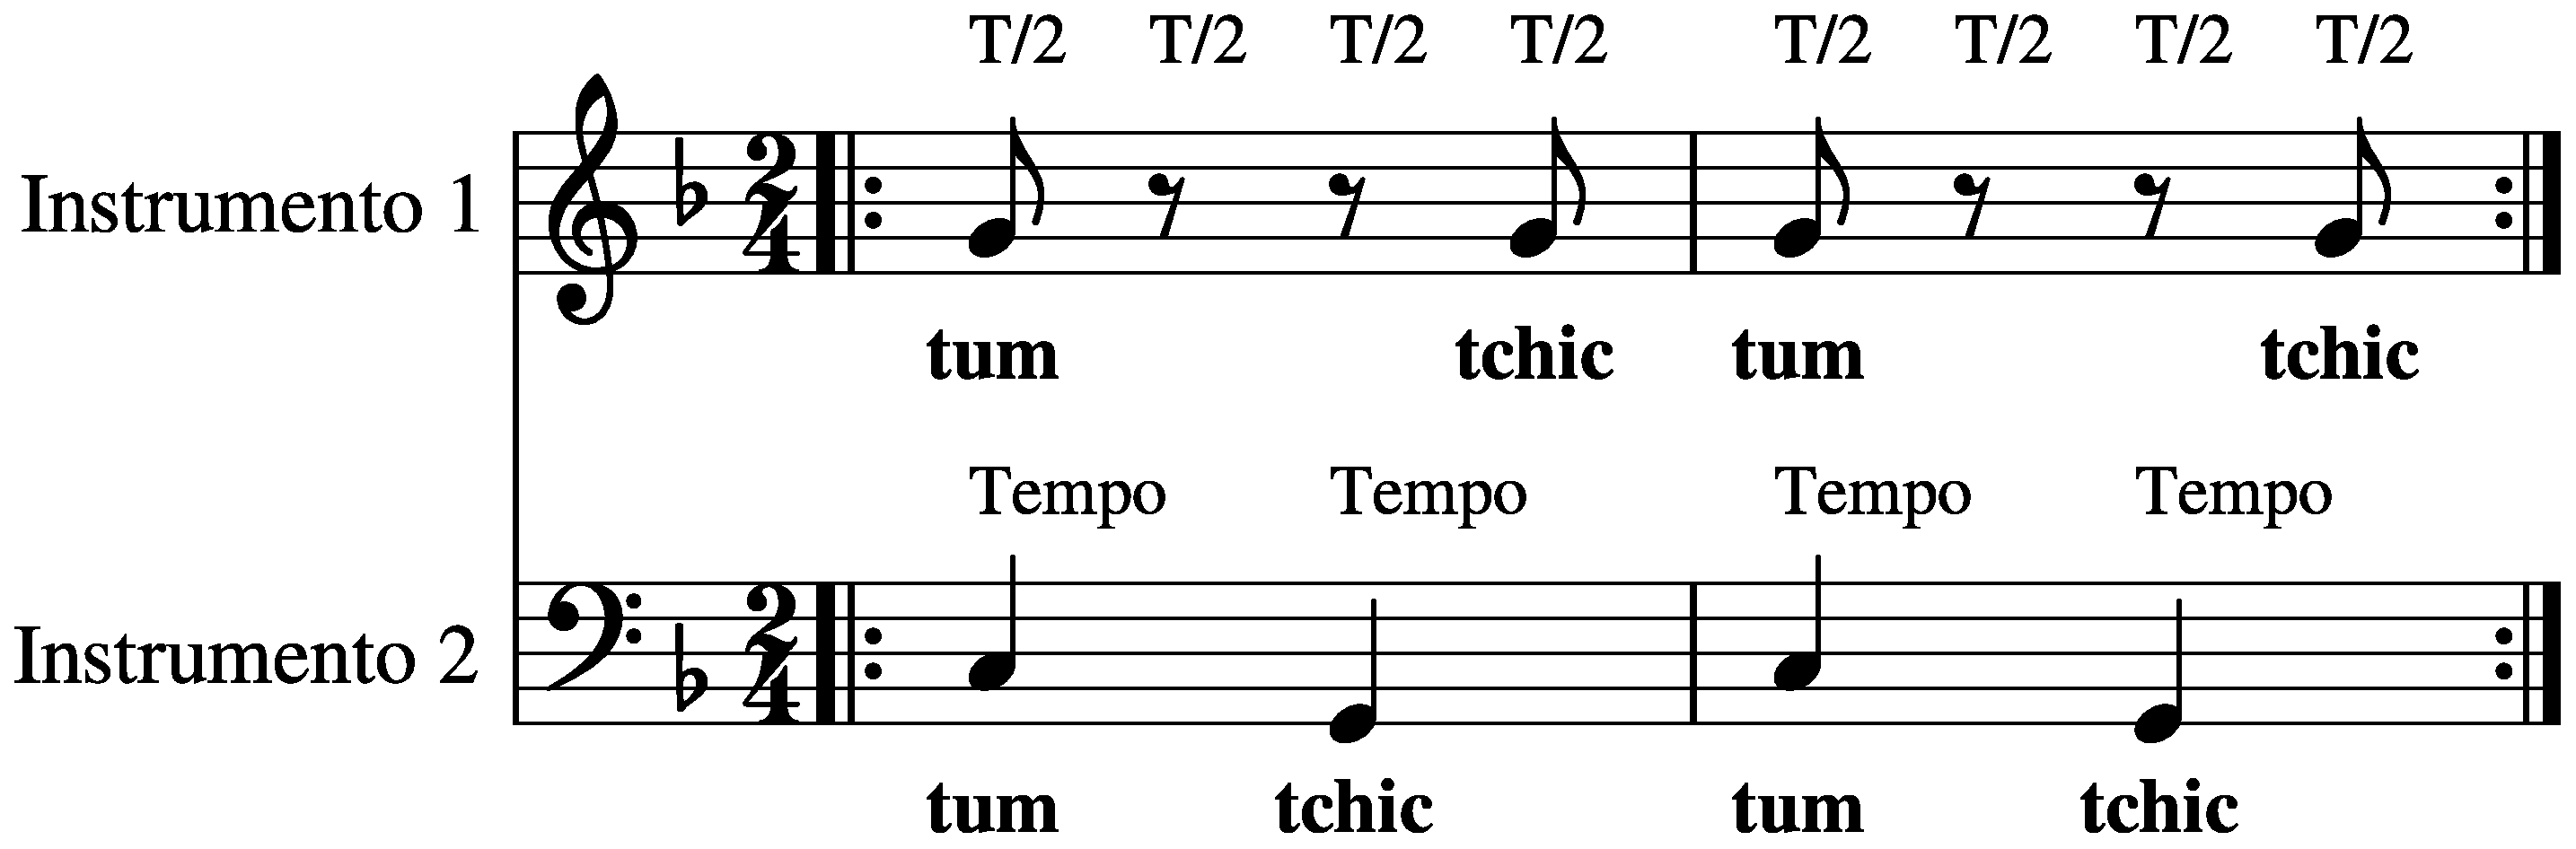
\includegraphics[width=0.8\textwidth]{chapters/cap-musicalidade-percepcion/abc-tchic-tchic-tum-1.eps}}
\begin{comment}
\begin{abc}[name=abc-tchic-tchic-tum-1,width=0.75\linewidth]
X: 1 % start of header
K: C % scale: C major
M:2/4
%T: Contratempo num compasso binário
V:1 clef=treble name="Instrumento 1" sname="Inst. 1"
V:2 clef=bass   name="Instrumento 2" sname="Inst. 2"
[V:1] |: " ""T/2"G1 " ""T/2"z1 " ""T/2"z1 " ""T/2"G1 | " ""T/2"G1 " ""T/2"z1 " ""T/2"z1 " ""T/2"G1  :|
w:    tum                tchic                       tum                   tchic           
[V:2] |:  "Tempo"C,2 "Tempo"G,,2  | "Tempo"C,2 "Tempo"G,,2  :|
w:    tum       tchic              tum       tchic            
\end{abc}
\end{comment}
\caption{Padrão de repetição para gerar um sonido de onomatopeia ``tchic tchic tum''.}
\label{fig:abc-tchic-tchic-tum-1}
\end{figure}
Na qual o instrumento 1 executa dois sonidos, de modo que o primeiro contribui ao sonido 
``tum'' e o segundo sonido gera o segundo ``tchic'' do compasso; por outro lado,
o instrumento 2 executa um ritmo com um padrão
de repetição de dois sonidos ``tum'' e ``tchic'', nesse ordem;
sendo que a nota executada no tempo forte produz um sonido mais agudo que a 
executada no tempo fraco, isto é assim para poder diferenciar melhor ambos tempos.

\begin{figure}[!h]
\begin{elaboracion}{Samba: ``tchic tchic tum'' vs. métrica}
\index{Música!Ritmo vs. Fala}
Quando reconhecemos a onomatopeia ``tchic tchic tum'' no ritmo do samba, 
podemos perceber que existe uma confusão entre 
a forma que é escrita ou encaixada esta onomatopeia na partitura e como achamos que é ao escutar ela.
Pois como é visto na Figura \ref{fig:abc-tchic-tchic-tum-1}, quando escrevemos
um ritmo cíclico com um padrão de repetição na ordem ``tum tchic tchic'' (|:\Vier \Acht \Acht:|) 
para o ouvinte é mais natural pensar que se está executando um ritmo com um padrão ``tchic tchic tum'' 
(|:\Acht \Acht \Vier:|), 
devido a que quando um ser humano fala, este usa a pausa
para denotar o final de uma palavra dado um conjunto de sílabas. Assim, ao escutar o padrão ``tum tchic tchic'', 
nossa mente otimizada para detetar palavras associa o sonido que tem um silencio maior apos ser executado,
neste caso o ``tum'' (a sílaba), com a posição final do ciclo do padrão de repetição (a palavra). 

Pelo que quando um músico vê um padrão de repetição ``tum tchic tchic'' na partitura; 
um ouvinte interpretará de forma instintiva que o padrão é ``tchic tchic tum'' iniciando em ``tchic''.
Porém não devemos confundir-nos, o ``tum'' é executado no tempo 1 do compasso.
\end{elaboracion}
\label{fig:RitmoVsFala}
\end{figure}

\subsection{Percepção do: tum~tum}

Analisando o fragmento de partitura da Figura \ref{fig:abc-caquarela} 
e tentando escutar os compassos 
para audivelmente isolar o instrumento ``D. Bass'',
podemos perceber que este gera um sonido 
com um \hyperref[sec:pos:Altura]{\textbf{tom}} muito grave, 
identificável com a onomatopeia ``tum tum'' e com uma duração de dois tempos.
No samba este ritmo é facilmente reconhecível na maioria das musicas 
e pode servi-nos de referencia quando dançamos ou quando simplesmente queremos achar o pulso.
Este instrumento é descrito isoladamente na Figura \ref{fig:abc-tum-tum-1},
na qual podemos apreciar que o compositor achou interessante diferenciar 
o tom do som que gerava o instrumento em cada tempo;
neste caso, um som mais agudo para o tempo forte e um mais grave para o tempo fraco;
porém esta diferença não é uma regra, pelo que se estamos procurando achar o tempo forte da música,
o melhor é simplesmente tentar perceber qual está sendo tocado com maior \hyperref[sec:pos:Intensidade]{\textbf{intensidade}}.
\begin{figure}[ht]
\centering
\href{https://drive.google.com/file/d/1uVEoBXD-itWcbqlr6CRrkShvS-ivBz7K/view?usp=sharing}{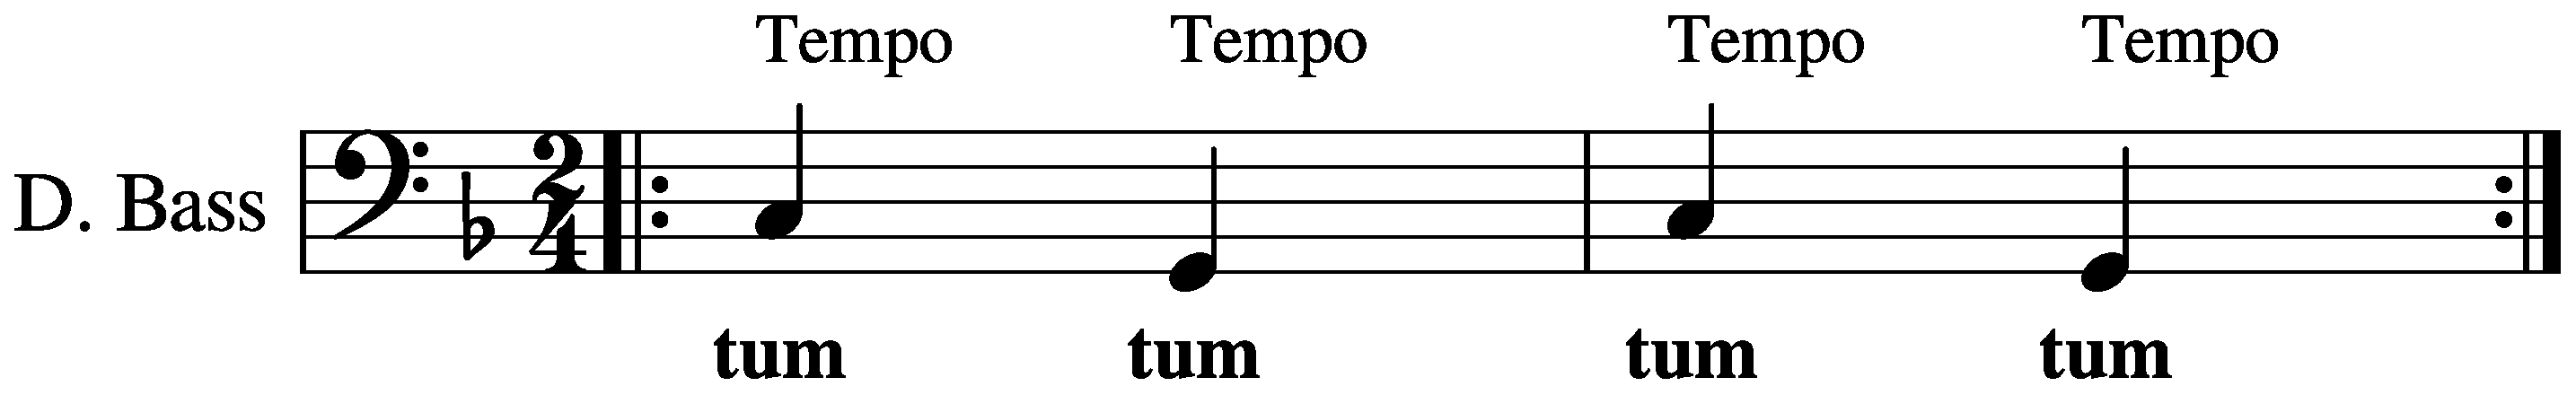
\includegraphics[width=0.9\textwidth]{chapters/cap-musicalidade-percepcion/abc-tum-tum-1.eps}}
\begin{comment}
\begin{abc}[name=abc-tum-tum-1,width=0.65\linewidth]
X: 1 % start of header
K: C % scale: C major
M:2/4
%T: Contratempo num compasso binário
V:1 clef=bass   name="D. Bass" sname="D. Bass"      
[V:1] |: "Tempo"C,2 "Tempo"G,,2  | "Tempo"C,2 "Tempo"G,,2  :|
w:    tum       tum         tum       tum            
\end{abc}
\end{comment}
\caption{Padrão de repetição para gerar um sonido de onomatopeia ``tum tum''.}
\label{fig:abc-tum-tum-1}
\end{figure}


%%%%%%%%%%%%%%%%%%%%%%%%%%%%%%%%%%%%%%%%%%%%%%%%%%%%%%%%%%%%%%%%%%%%%%%%%%%%%%%%
%%%%%%%%%%%%%%%%%%%%%%%%%%%%%%%%%%%%%%%%%%%%%%%%%%%%%%%%%%%%%%%%%%%%%%%%%%%%%%%%
\section{Percepção rítmica (exercícios)}
\index{Musicalidade!Percepção rítmica}



Como já foi visto na Seção \ref{sec:percepcaosamba1},
existem um conjunto de onomatopeias, que representam  tradicionalmente,
aos ritmos  que acompanham à melodia principal, 
nas músicas que pertencem aos \hyperref[sec:FamiliaSamba]{\textbf{subgêneros do samba}};
estes ritmos de acompanhamento, ou as simplificações que percebemos, 
geralmente tem um padrão muito homogêneo entre compassos sucessivos,
de modo que são muito fáceis de predizer para um dançarino, 
e estes podem servir de guia ou como um porto seguro.

Assim, esses ritmos simples, geralmente são usados como uma forma que emoldura a execução dos passos básicos,
e alguns mais complexos;
porem, existem passos ou movimentos no samba de gafieira e outros estilos de dança,
que se saem desses padrões rítmicos simples. 
\begin{itemize}
\item Em alguns casos,
isto é feito para agregar artisticamente um pouco de complexidade aos movimentos,
porem sem sair-nos completamente da guia do ritmo do acompanhamento; mas 
\item em outros casos, nos saímos dos padrões desse ritmo, 
porque deixamos de seguir o ritmo do acompanhamento,
e iniciamos a seguir o ritmo da melodia principal, que geralmente é mais complexa,
e muito heterogênea entre compassos sucessivos\footnote{Este 
tema será abordado mais amplamente na Seção \ref{sec:aspectosusicalidade}.}. 
\end{itemize}~


Nesta seção serão presentadas uma serie dinâmicas grupais, 
para decorar e acostuma-nos ao uso dos ritmos mais simples e comuns, 
a serem usados no acompanhamento do samba de gafieira e outros estilos de dança.

Nestos exemplos, está escrito com maiúscula a onomatopeia 
que cai no tempo com acento métrico, para lembrar este detalhe na execução do som. 
Também, além de uma pauta para descrever os exemplos, 
é desenhada uma representação num diagrama circular,
para facilitar a leitura e execução da pauta.
Nesse diagrama, os círculos pretos representam notas executadas em tempo forte,
e os círculos cinza, as notas executadas num tempo fraco;
a leitura do diagrama deve ser feito em sentido horário.  

\begin{example}[Treinamentos simples:]
Um professor, ou um software programado, 
deve executar, uma ou duas vesses, alguma das sequencias rítmicas mostradas nas Figuras 
\ref{fig:abc-percepcionritmica1}, \ref{fig:abc-percepcionritmica2},
\ref{fig:abc-percepcionritmica3}  e \ref{fig:abc-percepcionritmica4}.
Seguidamente os estudantes devem lembrar e repetir o ritmo, 
incluindo as acentuações, dando palmas ou batendo com os pés.
\end{example}


\begin{figure}[H]
\centering
     \begin{subfigure}[c]{0.45\textwidth}
         \centering
         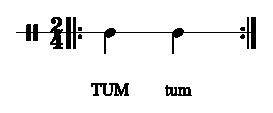
\includegraphics[width=\textwidth]{chapters/cap-musicalidade-percepcion/treino-ritmo1-1.eps}
         \caption{Pauta do ritmo TUM tum.}
         \label{fig:RitmoTUMtum1}
     \end{subfigure}
     \hfill
     \begin{subfigure}[c]{0.45\textwidth}
         \centering
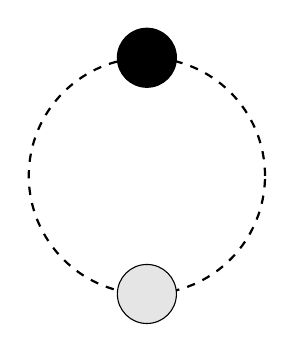
\begin{tikzpicture}
\pgfmathsetmacro{\RadioTot}{1.5}
\pgfmathsetmacro{\Base}{4}
\pgfmathsetmacro{\Radio}{\RadioTot/\Base}
\pgfmathsetmacro{\Theta}{360/\Base}

\draw[black,thick,dashed] (0,0) circle (\RadioTot cm);

\foreach \x in {2}
{
	\draw  [black,fill=gray!20] ({\RadioTot*cos(90-\x*\Theta )} ,{\RadioTot*sin(90-\x*\Theta )})circle (\Radio cm);
}

\foreach \x in {0}
{
	\draw  [black,fill=black] ({\RadioTot*cos(90-\x*\Theta )} ,{\RadioTot*sin(90-\x*\Theta )})circle (\Radio cm);
}
\end{tikzpicture}
         \caption{Diagrama circular do ritmo TUM tum.}
         \label{fig:RitmoTUMtum2}
     \end{subfigure}
\caption{Descrição do ritmo ``TUM tum''.}
\label{fig:abc-percepcionritmica1}
\end{figure}


\begin{figure}[H]
\centering
     \begin{subfigure}[c]{0.45\textwidth}
         \centering
         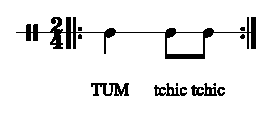
\includegraphics[width=\textwidth]{chapters/cap-musicalidade-percepcion/treino-ritmo2-1.eps}
         \caption{Pauta do ritmo TUM tchic tchic.}
         \label{fig:RitmoTUMtchictchic1}
     \end{subfigure}
     \hfill
     \begin{subfigure}[c]{0.45\textwidth}
         \centering
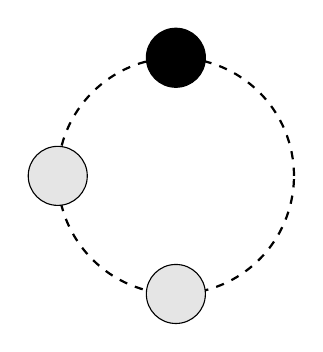
\begin{tikzpicture}
\pgfmathsetmacro{\RadioTot}{1.5}
\pgfmathsetmacro{\Base}{4}
\pgfmathsetmacro{\Radio}{\RadioTot/\Base}
\pgfmathsetmacro{\Theta}{360/\Base}

\draw[black,thick,dashed] (0,0) circle (\RadioTot cm);

\foreach \x in {2,3}
{
	\draw  [black,fill=gray!20] ({\RadioTot*cos(90-\x*\Theta )} ,{\RadioTot*sin(90-\x*\Theta )})circle (\Radio cm);
}

\foreach \x in {0}
{
	\draw  [black,fill=black] ({\RadioTot*cos(90-\x*\Theta )} ,{\RadioTot*sin(90-\x*\Theta )})circle (\Radio cm);
}
\end{tikzpicture}
         \caption{Diagrama circular do ritmo TUM tchic tchic.}
         \label{fig:RitmoTUMtchictchic2}
     \end{subfigure}
\caption{Descrição do ritmo ``TUM tchic tchic''.}
\label{fig:abc-percepcionritmica2}
\end{figure}

\begin{figure}[H]
\centering
     \begin{subfigure}[c]{0.45\textwidth}
         \centering
         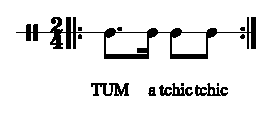
\includegraphics[width=\textwidth]{chapters/cap-musicalidade-percepcion/treino-ritmo3-1.eps}
         \caption{Pauta do ritmo TUM a tchic tchic.}
         \label{fig:RitmoTUMatchictchic1}
     \end{subfigure}
     \hfill
     \begin{subfigure}[c]{0.45\textwidth}
         \centering
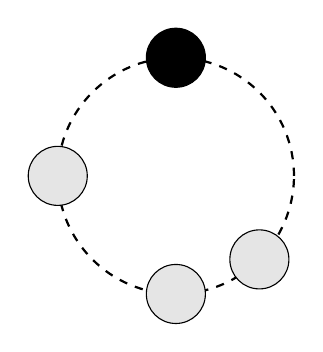
\begin{tikzpicture}
\pgfmathsetmacro{\RadioTot}{1.5}
\pgfmathsetmacro{\Base}{4}
\pgfmathsetmacro{\Radio}{\RadioTot/\Base}
\pgfmathsetmacro{\Theta}{360/\Base}

\draw[black,thick,dashed] (0,0) circle (\RadioTot cm);

\foreach \x in {1.5,2,3}
{
	\draw  [black,fill=gray!20] ({\RadioTot*cos(90-\x*\Theta )} ,{\RadioTot*sin(90-\x*\Theta )})circle (\Radio cm);
}

\foreach \x in {0}
{
	\draw  [black,fill=black] ({\RadioTot*cos(90-\x*\Theta )} ,{\RadioTot*sin(90-\x*\Theta )})circle (\Radio cm);
}
\end{tikzpicture}
         \caption{Diagrama circular do ritmo TUM a tchic tchic.}
         \label{fig:RitmoTUMatchictchic2}
     \end{subfigure}
\caption{Descrição do ritmo ``TUM a tchic tchic''.}
\label{fig:abc-percepcionritmica3}
\end{figure}


\begin{figure}[H]
\centering
     \begin{subfigure}[c]{0.45\textwidth}
         \centering
         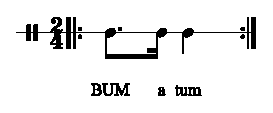
\includegraphics[width=\textwidth]{chapters/cap-musicalidade-percepcion/treino-ritmo4-1.eps}
         \caption{Pauta do ritmo TUM a tum.}
         \label{fig:RitmoTUMatum1}
     \end{subfigure}
     \hfill
     \begin{subfigure}[c]{0.45\textwidth}
         \centering
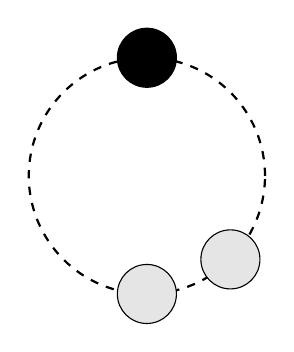
\begin{tikzpicture}
\pgfmathsetmacro{\RadioTot}{1.5}
\pgfmathsetmacro{\Base}{4}
\pgfmathsetmacro{\Radio}{\RadioTot/\Base}
\pgfmathsetmacro{\Theta}{360/\Base}

\draw[black,thick,dashed] (0,0) circle (\RadioTot cm);

\foreach \x in {1.5,2}
{
	\draw  [black,fill=gray!20] ({\RadioTot*cos(90-\x*\Theta )} ,{\RadioTot*sin(90-\x*\Theta )})circle (\Radio cm);
}

\foreach \x in {0}
{
	\draw  [black,fill=black] ({\RadioTot*cos(90-\x*\Theta )} ,{\RadioTot*sin(90-\x*\Theta )})circle (\Radio cm);
}
\end{tikzpicture}
         \caption{Diagrama circular do ritmo TUM a tum.}
         \label{fig:RitmoTUMatum2}
     \end{subfigure}
\caption{Descrição do ritmo ``TUM a tum''.}
\label{fig:abc-percepcionritmica4}
\end{figure}

\begin{example}[Treinamentos elaborados:]
Um professor, ou um software programado, 
deve executar muitas vesses, por exemplo 32, 
as sequencias rítmicas mostradas nas Figuras 
\ref{fig:abc-percepcionritmica5} e \ref{fig:abc-percepcionritmica6}.
Enquanto que os estudantes acompanham o ritmo, 
incluindo as acentuações, dando palmas ou batendo com os pés\footnote{Pode
ser divertido indicar que se pode andar e criar movimentos com os pés, 
sempre que se respeite o ritmo proposto.},
de jeito que a sincronia seja perfeita.
\end{example}

\begin{figure}[H]
\centering
     \begin{subfigure}[c]{0.45\textwidth}
         \centering
         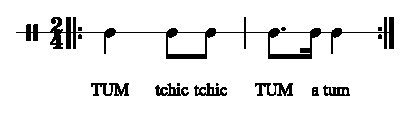
\includegraphics[width=\textwidth]{chapters/cap-musicalidade-percepcion/treino-ritmo5-1.eps}
         \caption{Pauta do ritmo.}
         \label{fig:Ritmocomplexo1:1}
     \end{subfigure}
     \hfill
     \begin{subfigure}[c]{0.45\textwidth}
         \centering
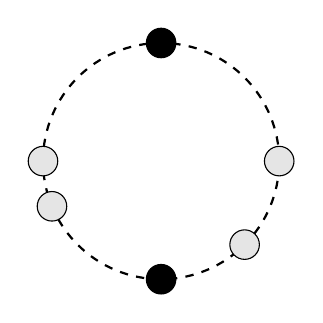
\begin{tikzpicture}
\pgfmathsetmacro{\RadioTot}{1.5}
\pgfmathsetmacro{\Base}{8}
\pgfmathsetmacro{\Radio}{\RadioTot/\Base}
\pgfmathsetmacro{\Theta}{360/\Base}

\draw[black,thick,dashed] (0,0) circle (\RadioTot cm);

\foreach \x in {2,3,5.5,6}
{
	\draw  [black,fill=gray!20] ({\RadioTot*cos(90-\x*\Theta )} ,{\RadioTot*sin(90-\x*\Theta )})circle (\Radio cm);
}

\foreach \x in {0,4}
{
	\draw  [black,fill=black] ({\RadioTot*cos(90-\x*\Theta )} ,{\RadioTot*sin(90-\x*\Theta )})circle (\Radio cm);
}
\end{tikzpicture}
         \caption{Diagrama circular do ritmo.}
         \label{fig:Ritmocomplexo1:2}
     \end{subfigure}
\caption{Descrição do ritmo.}
\label{fig:abc-percepcionritmica5}
\end{figure}





\begin{figure}[H]
\centering
     \begin{subfigure}[c]{0.45\textwidth}
         \centering
         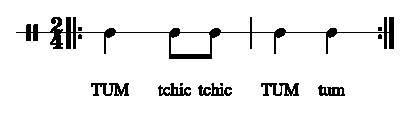
\includegraphics[width=\textwidth]{chapters/cap-musicalidade-percepcion/treino-ritmo6-1.eps}
         \caption{Pauta do ritmo.}
         \label{fig:Ritmocomplexo2:1}
     \end{subfigure}
     \hfill
     \begin{subfigure}[c]{0.45\textwidth}
         \centering
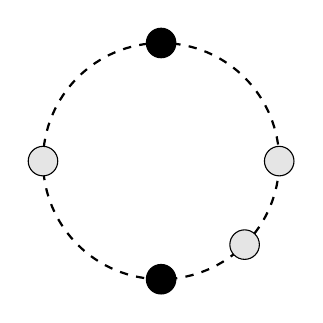
\begin{tikzpicture}
\pgfmathsetmacro{\RadioTot}{1.5}
\pgfmathsetmacro{\Base}{8}
\pgfmathsetmacro{\Radio}{\RadioTot/\Base}
\pgfmathsetmacro{\Theta}{360/\Base}

\draw[black,thick,dashed] (0,0) circle (\RadioTot cm);

\foreach \x in {2,3,6}
{
	\draw  [black,fill=gray!20] ({\RadioTot*cos(90-\x*\Theta )} ,{\RadioTot*sin(90-\x*\Theta )})circle (\Radio cm);
}

\foreach \x in {0,4}
{
	\draw  [black,fill=black] ({\RadioTot*cos(90-\x*\Theta )} ,{\RadioTot*sin(90-\x*\Theta )})circle (\Radio cm);
}
\end{tikzpicture}
         \caption{Diagrama circular do ritmo.}
         \label{fig:Ritmocomplexo2:2}
     \end{subfigure}
\caption{Descrição do ritmo.}
\label{fig:abc-percepcionritmica6}
\end{figure}


%\section{Reconhecendo o tom}
% \cite[pp. 116]{alves2004teoria}

